% !TeX program = xelatex
\documentclass[a4paper,12pt]{article}

% ===== 1. KHỔ GIẤY, LỀ TRANG, FONT =====
\usepackage[left=3cm,right=2cm,top=2cm,bottom=2cm,footskip=1cm]{geometry}
\usepackage{fontspec}

\IfFontExistsTF{Times New Roman}{
  \setmainfont{Times New Roman}
}{
  \IfFileExists{fonts/times.ttf}{
    \setmainfont{times.ttf}[
      Path=fonts/,
      BoldFont=timesbd.ttf,
      ItalicFont=timesi.ttf,
      BoldItalicFont=timesbi.ttf]
  }{
    \IfFontExistsTF{TeX Gyre Termes}{
      \setmainfont{TeX Gyre Termes}
      \PackageWarningNoLine{MauBaoCao}{Times New Roman unavailable; using TeX Gyre Termes}
    }{
      \setmainfont{DejaVu Serif}
      \PackageWarningNoLine{MauBaoCao}{Times New Roman unavailable; using DejaVu Serif}
    }
  }
}
\usepackage{indentfirst}
\usepackage{microtype}
\usepackage{graphicx}
\usepackage{float}
\usepackage{tikz}
\usepackage{array,tabularx,booktabs,longtable}
\usepackage{enumitem}
\usepackage{titlesec}
\usepackage{tocloft}
\usepackage{caption}
\usepackage{xurl}
\usepackage[unicode,hidelinks]{hyperref}
\urlstyle{same}

\renewcommand{\normalsize}{\fontsize{13}{19.5}\selectfont}
\AtBeginDocument{\normalsize}
\setlength{\parindent}{0.5cm}
\setlength{\parskip}{4pt}
\setlength{\emergencystretch}{2em}
\raggedbottom
\setlist{topsep=4pt,itemsep=2pt,parsep=0pt,leftmargin=*}

% ===== 2. BA CẤP TIÊU ĐỀ: 1 / 1.1 / 1.1.1 =====
\setcounter{secnumdepth}{3}
\setcounter{tocdepth}{3}
\renewcommand{\thesection}{\arabic{section}}
\renewcommand{\thesubsection}{\thesection.\arabic{subsection}}
\renewcommand{\thesubsubsection}{\thesubsection.\arabic{subsubsection}}
\titleformat{\section}[hang]
  {\normalfont\fontsize{16}{20}\selectfont\bfseries}
  {\thesection.}{0.6em}{}
\titleformat{\subsection}[hang]
  {\normalfont\fontsize{14}{18}\selectfont\bfseries}
  {\thesubsection}{0.6em}{}
\titleformat{\subsubsection}[hang]
  {\normalfont\fontsize{13}{17}\selectfont\bfseries}
  {\thesubsubsection}{0.6em}{}
\titlespacing*{\section}{0pt}{16pt}{8pt}
\titlespacing*{\subsection}{0pt}{12pt}{6pt}
\titlespacing*{\subsubsection}{0pt}{8pt}{4pt}

% ===== 3. MỤC LỤC VÀ SỐ TRANG =====
\renewcommand{\contentsname}{MỤC LỤC}
\renewcommand{\refname}{Tài liệu tham khảo}
\renewcommand{\cfttoctitlefont}{\fontsize{16}{20}\selectfont\bfseries}
\setlength{\cftbeforetoctitleskip}{0pt}
\setlength{\cftaftertoctitleskip}{18pt}
\renewcommand{\cftsecfont}{\normalfont\bfseries}
\renewcommand{\cftsecpagefont}{\normalfont\bfseries}
\renewcommand{\cftsubsecfont}{\normalfont}
\renewcommand{\cftsubsubsecfont}{\normalfont}
\renewcommand{\cftsecleader}{\cftdotfill{\cftdotsep}}
\cftsetindents{section}{0em}{2em}
\cftsetindents{subsection}{2em}{3em}
\cftsetindents{subsubsection}{5em}{4em}
\setlength{\cftbeforesecskip}{6pt}
\makeatletter
\def\ps@plain{%
  \let\@oddhead\@empty\let\@evenhead\@empty
  \def\@oddfoot{\hfil{\normalfont\fontsize{11}{13}\selectfont\thepage}\hfil}%
  \let\@evenfoot\@oddfoot}
\makeatother
\pagestyle{plain}

% ===== 4. BẢNG, HÌNH, CHÚ THÍCH =====
\renewcommand{\tablename}{Bảng}
\renewcommand{\figurename}{Hình}
\DeclareCaptionFont{reportcaption}{\fontsize{12}{15}\selectfont}
\captionsetup{font=reportcaption,labelfont=bf,labelsep=period,
  justification=centering,skip=6pt}
\newcolumntype{Y}{>{\raggedright\arraybackslash}X}
\newcommand{\bangfont}{\fontsize{12}{15}\selectfont}
\newcommand{\code}[1]{\texttt{#1}}

% ===== 5. THÔNG TIN TRANG BÌA =====
\newcommand{\DonViChuQuan}{ĐẠI HỌC QUỐC GIA HÀ NỘI}
\newcommand{\TenTruong}{TRƯỜNG ĐẠI HỌC CÔNG NGHỆ}
\newcommand{\LoaiBaoCao}{BÁO CÁO CUỐI KỲ}
\newcommand{\TenMonHoc}{ĐIỆN TOÁN ĐÁM MÂY}
\newcommand{\TenDeTai}{SatiBot -- Quản lý và tương tác với các tài nguyên AWS bằng ngôn ngữ tự nhiên}
\newcommand{\GiangVien}{TS. Hoàng Xuân Tùng}
\newcommand{\SoNhom}{Nhóm 10}
\newcommand{\LopMonHoc}{INT3319 1}
\newcommand{\DiaDiemThoiGian}{Hà Nội, Tháng 11/2026}
\hypersetup{pdftitle={BÁO CÁO CUỐI KỲ - SATIBOT},pdfauthor={Nhóm 10}}

\begin{document}

% ===== 6. TRANG BÌA =====
\begin{titlepage}
\thispagestyle{empty}
\begin{tikzpicture}[remember picture,overlay]
  \draw[line width=2pt]
    ([xshift=3cm,yshift=-2cm]current page.north west)
    rectangle ([xshift=-2cm,yshift=2cm]current page.south east);
  \draw[line width=0.5pt]
    ([xshift=3.12cm,yshift=-2.12cm]current page.north west)
    rectangle ([xshift=-2.12cm,yshift=2.12cm]current page.south east);
\end{tikzpicture}\par
\centering
\setlength{\parindent}{0pt}
\setlength{\parskip}{0pt}
\vspace*{0.8cm}
{\fontsize{14}{18}\selectfont\bfseries\DonViChuQuan\par}
\vspace{0.15cm}
{\fontsize{15}{20}\selectfont\bfseries\TenTruong\par}
\vspace{0.25cm}
\rule{5cm}{0.4pt}\par
\vspace{0.5cm}

\IfFileExists{logo.png}{
  
\includegraphics[width=3.8cm,height=3.8cm,keepaspectratio]{logo.png}
}{
  \IfFileExists{Report progress 2/logo.png}{
    \includegraphics[width=3.8cm,height=3.8cm,keepaspectratio]{Report progress 2/logo.png}
  }{
    \IfFileExists{Report progress 1/logo.png}{
      \includegraphics[width=3.8cm,height=3.8cm,keepaspectratio]{Report progress 1/logo.png}
    }{
      \fbox{\parbox[c][3.4cm][c]{3.4cm}{\centering
        \fontsize{11}{14}\selectfont LOGO TRƯỜNG}}
    }
  }
}\par
\vspace{0.7cm}
{\fontsize{22}{27}\selectfont\bfseries\LoaiBaoCao\par}
\vspace{0.35cm}
\begin{minipage}{0.9\textwidth}\centering
  {\fontsize{15}{20}\selectfont\bfseries MÔN HỌC: \TenMonHoc\par}
\end{minipage}\par
\vspace{0.6cm}
{\fontsize{13}{17}\selectfont\bfseries ĐỀ TÀI\par}
\vspace{0.12cm}
\begin{minipage}{0.9\textwidth}\centering
  {\fontsize{16}{21}\selectfont\bfseries\TenDeTai\par}
\end{minipage}\par
\vspace{0.65cm}
{\fontsize{13}{19.5}\selectfont
\renewcommand{\arraystretch}{1.1}
\begin{tabular}{@{}>{\raggedright\arraybackslash\bfseries}p{5.2cm}>{\raggedright\arraybackslash}p{8cm}@{}}
  Giảng viên hướng dẫn: & \GiangVien\\
  Nhóm thực hiện: & \SoNhom\\
  Sinh viên thực hiện: & Cao Anh Minh \textbf{(Trưởng nhóm)}\\
                      & Trịnh Thiên Quang\\
                      & Phạm Đức Hùng\\
                      & Nguyễn Đức Huy\\
  Lớp môn học: &  \LopMonHoc
\end{tabular}\par}
\vfill
{\fontsize{13}{17}\selectfont\bfseries\DiaDiemThoiGian\par}
\vspace*{0.5cm}
\end{titlepage}

% ===== 7. MỤC LỤC TỰ ĐỘNG =====
\pagenumbering{roman}
\tableofcontents
\clearpage
\pagenumbering{arabic}

% ===== 8. NỘI DUNG BÁO CÁO =====

\section{TỔNG QUAN VỀ DỰ ÁN}

\subsection{Giới thiệu chung về tính năng dự án}

Hiện nay, Amazon Web Services (AWS) là một trong những nền tảng điện toán đám mây phổ biến nhất phục vụ học tập, nghiên cứu và triển khai ứng dụng. Tuy nhiên, việc khởi tạo và quản trị tài nguyên thông qua giao diện web (AWS Management Console) đòi hỏi nhiều thao tác thủ công, điều hướng qua nhiều màn hình cấu hình phức tạp và rất dễ nhầm lẫn. Trong khi đó, việc sử dụng giao diện dòng lệnh (AWS CLI) hoặc viết tập lệnh tự động lại yêu cầu ghi nhớ chính xác cú pháp câu lệnh, cấu trúc tệp cấu hình JSON và các tham số kỹ thuật. Đối với sinh viên, lập trình viên mới tiếp cận điện toán đám mây hoặc người quản lý kỹ thuật, các rào cản này làm chậm quá trình vận hành, đồng thời tiềm ẩn nguy cơ cấu hình sai gây mất an toàn thông tin hoặc phát sinh chi phí ngoài ý muốn.

Nhằm giải quyết vấn đề trên, nhóm thực hiện đề tài xây dựng SatiBot -- ứng dụng ChatOps hỗ trợ quản lý, cấu hình và giám sát tài nguyên AWS thông qua câu lệnh bằng ngôn ngữ tự nhiên tiếng Việt. Bằng cách kết hợp mô hình ngôn ngữ lớn (LLM) hỗ trợ cơ chế \textit{Function Calling} với thư viện AWS SDK (Boto3), SatiBot hoạt động như một trợ lý hỗ trợ thao tác hạ tầng. Người dùng chỉ cần gửi yêu cầu bằng tiếng Việt qua giao diện chat; hệ thống sẽ phân tích ý định, kiểm tra tính hợp lệ và độ an toàn của câu lệnh, sau đó gọi các API tương ứng của AWS và trả về kết quả thực thi kèm theo thông tin chi tiết, cảnh báo rủi ro hoặc hướng dẫn xử lý tiếp theo.

\subsection{Giới thiệu người dùng của dự án}

Hệ thống SatiBot hướng tới 03 nhóm người dùng chính với nhu cầu sử dụng thực tế như sau:

\begin{itemize}
  \item \textbf{Lập trình viên và kỹ sư vận hành (Developers / DevOps Engineers):} Cần khởi tạo nhanh môi trường thử nghiệm, cấu hình máy chủ, cập nhật mã nguồn hàm serverless hoặc xem log hệ thống trong quá trình phát triển ứng dụng. SatiBot giúp nhóm này thực hiện các tác vụ lặp đi lặp lại nhanh hơn ngay trên khung chat mà không cần chuyển đổi qua lại giữa nhiều trang trên AWS Console.
  \item \textbf{Sinh viên ngành Công nghệ thông tin / Điện toán đám mây:} Cần môi trường thực hành trực quan cho các môn học về mạng và hạ tầng đám mây. Hệ thống cung cấp cơ chế kiểm tra an toàn (guardrails), giúp sinh viên tránh các lỗi phổ biến như mở cổng mạng công khai nguy hiểm, quên tắt máy ảo hoặc chọn nhầm các gói cấu hình vượt quá phạm vi gói miễn phí (AWS Free Tier).
  \item \textbf{Quản lý kỹ thuật và chủ dự án (Tech Leads / Project Managers):} Cần theo dõi nhanh tình trạng hoạt động của tài nguyên, kiểm tra phân quyền (IAM Audit) và kiểm soát chi phí sử dụng hàng tháng (FinOps) bằng ngôn ngữ tự nhiên mà không cần thành thạo cú pháp dòng lệnh AWS CLI.
\end{itemize}

\subsection{Các dịch vụ AWS được hỗ trợ trong dự án}

\begingroup
\setlist{topsep=2pt,itemsep=1pt,parsep=0pt,leftmargin=*}
\setlength{\parskip}{2pt}

Để đáp ứng nhu cầu quản trị hạ tầng cơ bản, SatiBot hỗ trợ 04 dịch vụ chính của AWS gồm: Amazon EC2, Amazon S3, AWS IAM và AWS Lambda. Dưới đây là chi tiết về mục đích và quy trình tương tác thực tế của người dùng đối với từng nhóm tính năng của 04 dịch vụ AWS nòng cốt.

\subsubsection{Nhóm kịch bản Amazon EC2}

Dịch vụ máy chủ ảo (Amazon Elastic Compute Cloud - EC2) là hạ tầng phục vụ việc triển khai và chạy ứng dụng. SatiBot hỗ trợ 05 quy trình quản lý trạng thái và cấu hình máy ảo như sau:

\begin{enumerate}
  \item \textbf{Khởi tạo máy chủ chuẩn hóa và xử lý trùng lặp tên:}

Tạo nhanh máy ảo để thử nghiệm hoặc triển khai website mà không phải cấu hình thủ công nhiều bước, đồng thời xử lý trường hợp tên máy bị trùng.

  \item \textbf{Kiểm soát chi phí và xử lý vượt hạn mức tài nguyên (Cost Guardrails \& Quota):}

Tránh việc chọn nhầm máy cấu hình cao gây phát sinh chi phí lớn, đồng thời hướng dẫn cách xử lý khi tài khoản chạm ngưỡng hạn mức tạo máy ảo (vCPU quota).
  

  \item \textbf{Tra cứu và điều khiển vòng đời máy chủ (Bật / Tắt / Khởi động lại / Xóa):}

  Theo dõi danh sách máy ảo và điều khiển trạng thái bật/tắt kịp thời nhằm tránh lãng phí tài nguyên và kiểm soát chi phí vận hành.

  \item \textbf{Giám sát hiệu năng và phát hiện máy chủ lãng phí (FinOps \& CloudWatch):}

Theo dõi mức độ sử dụng tài nguyên để tắt các máy nhàn rỗi nhằm tiết kiệm chi phí, hoặc nhận biết máy bị quá tải để kịp thời nâng cấp.

  \item \textbf{Thiết lập tường lửa an toàn và hỗ trợ sự cố kết nối (SecOps):}

Bảo vệ máy chủ khỏi nguy cơ bị quét dò mật khẩu từ Internet (brute-force attack) và hỗ trợ chẩn đoán nhanh nguyên nhân khi không kết nối SSH được vào máy ảo.

\end{enumerate}

\subsubsection{Nhóm kịch bản Amazon S3}

Dịch vụ lưu trữ đối tượng (Amazon Simple Storage Service - S3) dùng để lưu trữ tập tin, bản sao lưu và dữ liệu tĩnh của hệ thống. SatiBot hỗ trợ 06 quy trình quản lý S3 như sau:

\begin{enumerate}
  \item \textbf{Khởi tạo thùng chứa (S3 Bucket) an toàn và chuẩn hóa:}

Tạo kho lưu trữ đối tượng được thiết lập ở chế độ riêng tư theo mặc định và tuân thủ quy tắc đặt tên của AWS.

  \item \textbf{Quét và khóa rủi ro lộ dữ liệu ra Internet (Security Scan \& Remediation):}

Rà soát và ngăn chặn kịp thời tình trạng lộ dữ liệu do vô tình mở quyền truy cập công khai (Public Access) trên bucket.


  \item \textbf{Xóa bucket S3 an toàn có kiểm soát (chống xóa nhầm dữ liệu):}

Dọn dẹp bucket cũ mà không lo ngại nguy cơ xóa nhầm dữ liệu quan trọng đang lưu bên trong.


  \item \textbf{Tối ưu chi phí lưu trữ lâu dài (FinOps Lifecycle Rules):}

Giảm thiểu chi phí lưu trữ bằng cách tự động chuyển các tệp cũ, ít sử dụng sang các tầng lưu trữ giá rẻ hơn (S3 Standard-IA, S3 Glacier).


  \item \textbf{Chia sẻ tệp tin an toàn có thời hạn (Presigned URL):}

  Cung cấp liên kết tải tệp tin an toàn cho người ngoài trong khoảng thời gian nhất định mà không cần mở public dữ liệu hay cấp quyền tài khoản AWS.


  \item \textbf{Tra cứu dung lượng và tình trạng kho lưu trữ (Storage Analytics):}

Nắm bắt nhanh số lượng tệp tin, dung lượng sử dụng thực tế và dự toán chi phí lưu trữ của từng bucket.

\end{enumerate}

\subsubsection{Nhóm kịch bản AWS IAM}

Dịch vụ quản lý định danh và quyền truy cập (AWS Identity and Access Management - IAM) là trung tâm kiểm soát an ninh của hạ tầng AWS. SatiBot cung cấp 05 quy trình quản trị IAM an toàn, tuân thủ nguyên tắc đặc quyền tối thiểu (Least Privilege):

\begin{enumerate}
  \item \textbf{Tra cứu vai trò (Role) và chính sách quyền hạn (Policy):}

Xem nhanh danh sách hoặc kiểm tra chi tiết các quyền hạn đang được gán cho nhân sự hoặc dịch vụ để phục vụ công tác kiểm toán an ninh.


  \item \textbf{Khởi tạo vai trò (Role) hoặc chính sách (Policy) mới theo nguyên tắc tối thiểu:}

Tạo mới đối tượng phân quyền cho máy chủ, ứng dụng hoặc nhân sự mà không phải tự tay viết các đoạn mã JSON chính sách phức tạp và dễ nhầm lẫn.


  \item \textbf{Cấp hoặc điều chỉnh quyền truy cập:}

Bổ sung hoặc nới rộng quyền hạn cho nhân sự/dịch vụ khi phát sinh công việc mới trong dự án.


  \item \textbf{Thu hồi quyền truy cập (Least Privilege Enforcement):}

Gỡ bỏ các quyền hạn không còn sử dụng hoặc thu hồi các quyền nguy hiểm (như quyền AdministratorAccess cấp thừa cho tài khoản thực tập sinh) nhằm hạn chế rủi ro an toàn thông tin.


  \item \textbf{Xóa đối tượng IAM an toàn:}

Dọn dẹp dứt điểm các Role, Policy hoặc User cũ không còn sử dụng để tránh dư thừa tài nguyên và loại bỏ lỗ hổng bảo mật tiềm tàng.

\end{enumerate}

\subsubsection{Nhóm kịch bản AWS Lambda}

Dịch vụ điện toán không máy chủ (AWS Lambda) cho phép chạy mã nguồn theo sự kiện. SatiBot hỗ trợ 05 quy trình quản trị và kiểm thử hàm serverless trực tiếp:

\begin{enumerate}
  \item \textbf{Tra cứu danh mục và kiểm tra cấu hình hàm (Inventory \& Config Audit):}

Nắm bắt nhanh toàn bộ các hàm Lambda đang có trong tài khoản cùng các thông số vận hành cốt lõi (ngôn ngữ runtime, bộ nhớ RAM, thời gian timeout) phục vụ công tác kiểm toán tài nguyên.


  \item \textbf{Chạy thử nghiệm hàm trực tiếp qua Chat (Direct Invocation):}

Kích hoạt và kiểm tra nhanh kết quả trả về của hàm với dữ liệu thử nghiệm ngay trên khung chat mà không cần đợi sự kiện bên ngoài hay cấu hình test event trên Console.


  \item \textbf{Điều chỉnh cấu hình bộ nhớ và thời gian chờ của hàm Lambda:}

Nâng cấp cấu hình tức thời cho các hàm đang chạy chậm hoặc có nguy cơ sập do thiếu bộ nhớ hay hết thời gian chờ mà không phải can thiệp mã nguồn hay mở Console.


  \item \textbf{Cấp phát nhanh liên kết HTTP công khai (Function URL Generation):}

Tạo nhanh một đường dẫn Endpoint HTTPS công khai (Function URL) để người dùng hoặc webhook bên ngoài có thể gọi trực tiếp hàm Lambda mà không mất công cấu hình API Gateway phức tạp.


  \item \textbf{Tạm dừng hoạt động hàm khẩn cấp (Emergency Kill-Switch):}

Vô hiệu hóa ngay lập tức một hàm đang bị lặp lỗi logic gây tiêu hao ngân sách hoặc cần ngắt kết nối gấp để bảo trì hệ thống mà không cần xóa bỏ mã nguồn của hàm.

\end{enumerate}
\endgroup

\clearpage

\section{GIẢI PHÁP THỰC HIỆN}

Chương này trình bày kiến trúc mục tiêu và các hợp đồng kỹ thuật của giải pháp.
Chương~3 đối chiếu thiết kế với các tài nguyên đã triển khai, kết quả kiểm thử
và những phần chưa được nghiệm thu trên tài khoản AWS mới.


\subsection{Kiến trúc tính năng của hệ thống}

\begin{figure}[H]
\centering
\IfFileExists{So_do_kien_truc_tinh_nang.jpg}{
  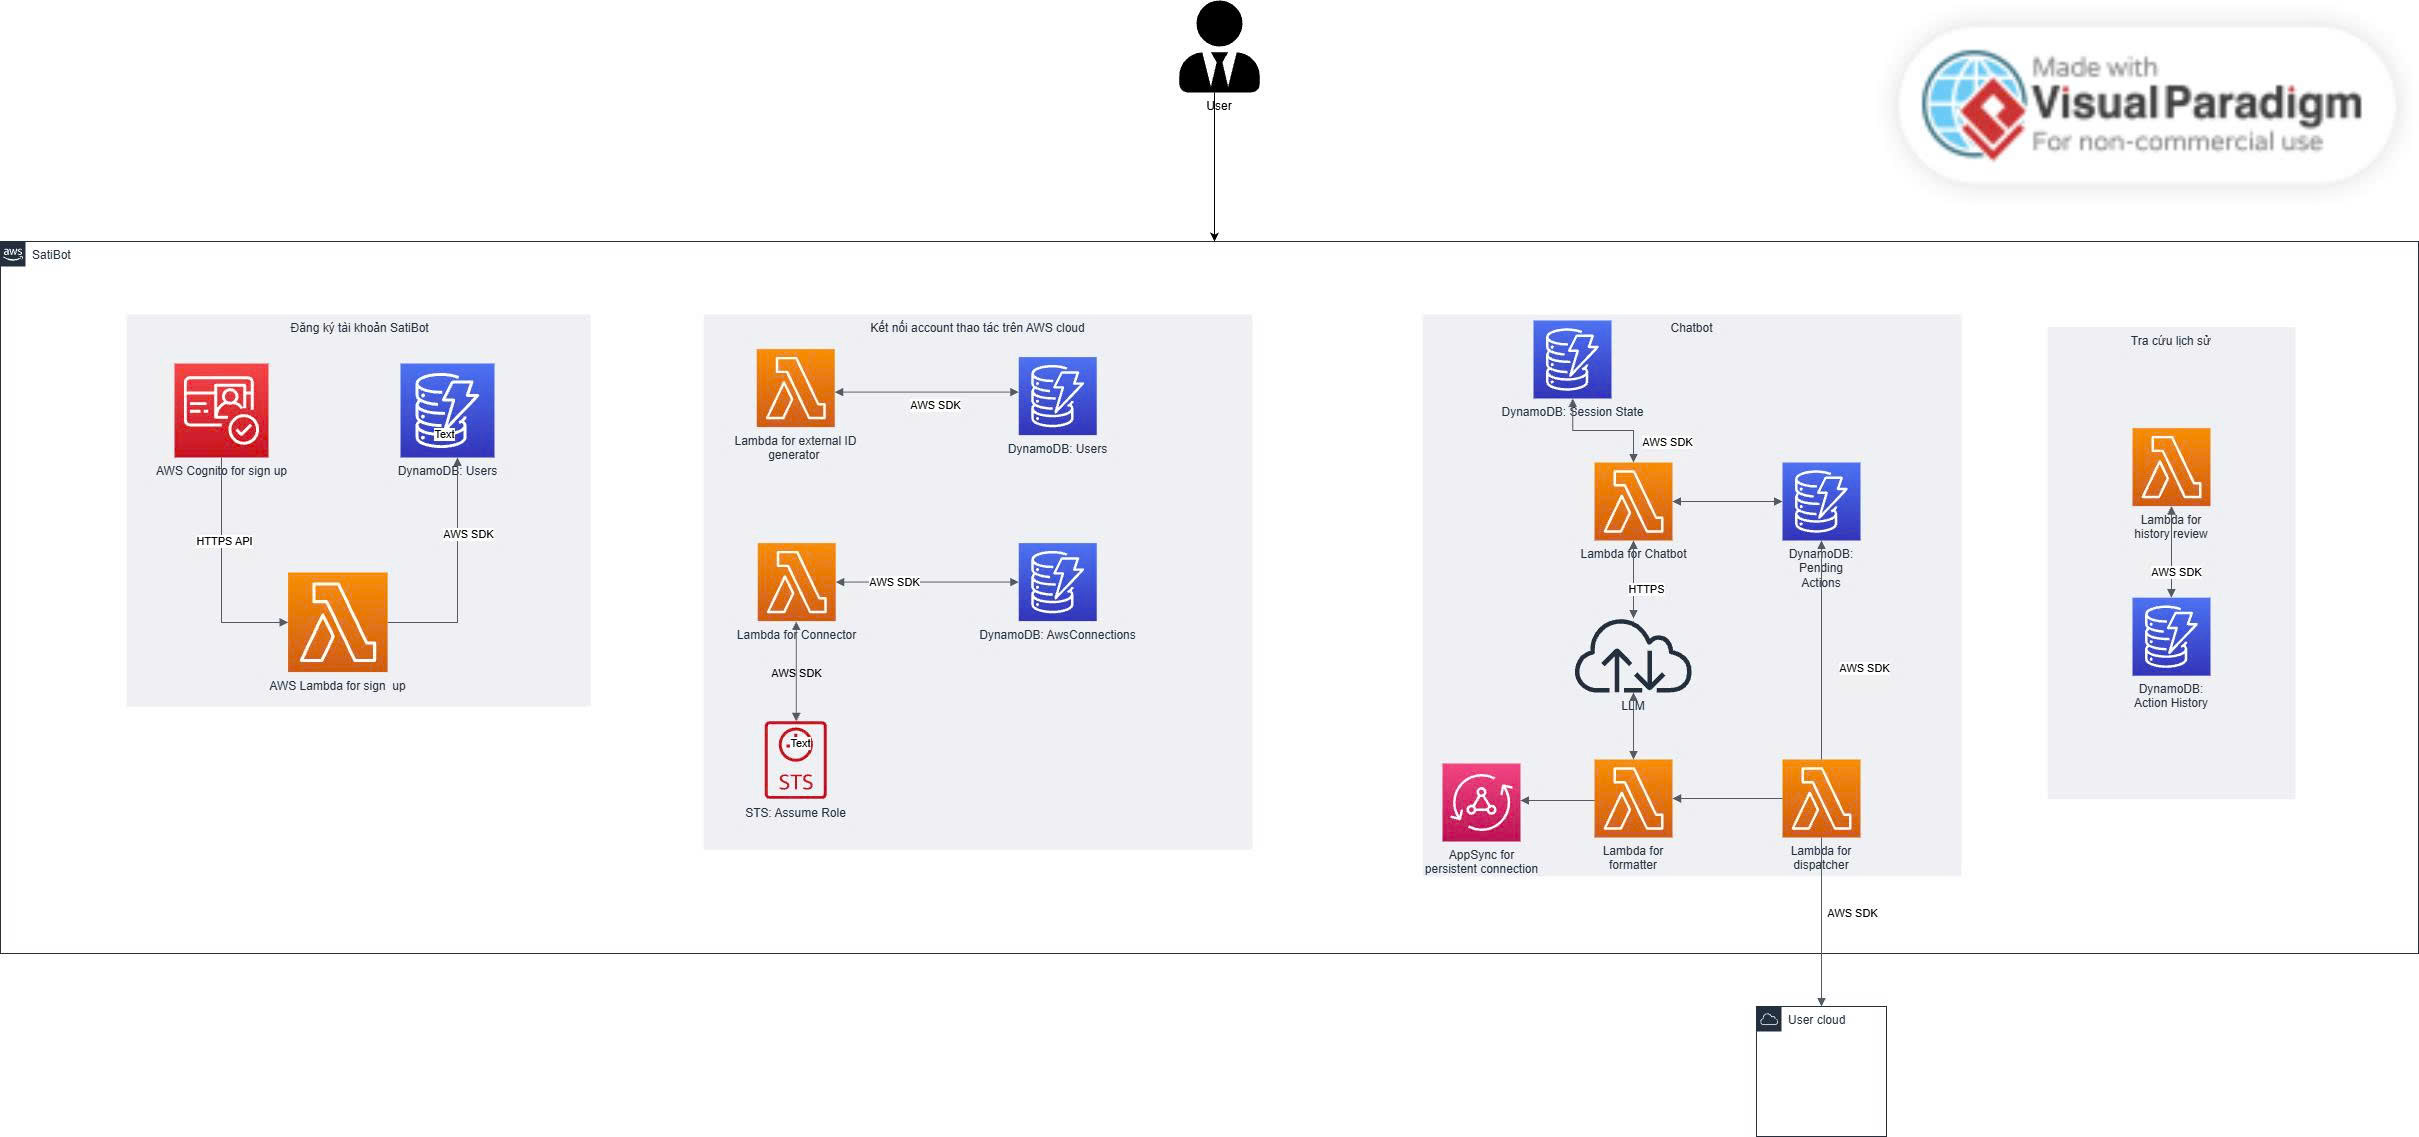
\includegraphics[width=0.8\textwidth]{So_do_kien_truc_tinh_nang.jpg}
}{
  \IfFileExists{Report progress 2/So_do_kien_truc_tinh_nang.jpg}{
    \includegraphics[width=0.8\textwidth]{Report progress 2/So_do_kien_truc_tinh_nang.jpg}
  }{
    \IfFileExists{Report progress 1/So_do_kien_truc_tinh_nang.jpg}{
      \includegraphics[width=0.8\textwidth]{Report progress 1/So_do_kien_truc_tinh_nang.jpg}
    }{
      \fbox{\parbox[c][6.5cm][c]{0.88\textwidth}{\centering Sơ đồ kiến trúc tính năng hệ thống SatiBot}}
    }
  }
}
\caption{Sơ đồ kiến trúc tính năng và luồng xử lý nghiệp vụ của SatiBot}
\label{fig:kientruc_tinhnang}
\end{figure}

Các tính năng hệ thống cung cấp bao gồm:
\begin{enumerate}[itemsep=3pt,topsep=2pt]
  \item \textbf{Đăng ký và xác thực người dùng:} Amazon Cognito xử lý đăng ký, đăng nhập và cấp JWT để xác thực các yêu cầu nghiệp vụ. Sau khi đăng ký, Lambda tạo hồ sơ người dùng trong bảng \texttt{Users} của DynamoDB.

  \item \textbf{Kết nối tài khoản AWS:} SatiBot tạo \texttt{ExternalId}; người dùng dùng mã này và hướng dẫn của hệ thống để tạo IAM Role trong tài khoản AWS của mình, sau đó gửi \texttt{RoleArn} về SatiBot. Connector Lambda gọi STS \texttt{AssumeRole} để kiểm tra khả năng ủy quyền. Nếu thành công, hệ thống lưu thông tin kết nối và trạng thái trong bảng \texttt{AwsConnections}.


  \begin{figure}[H]
  \centering
  \IfFileExists{sequence3.jpg}{
    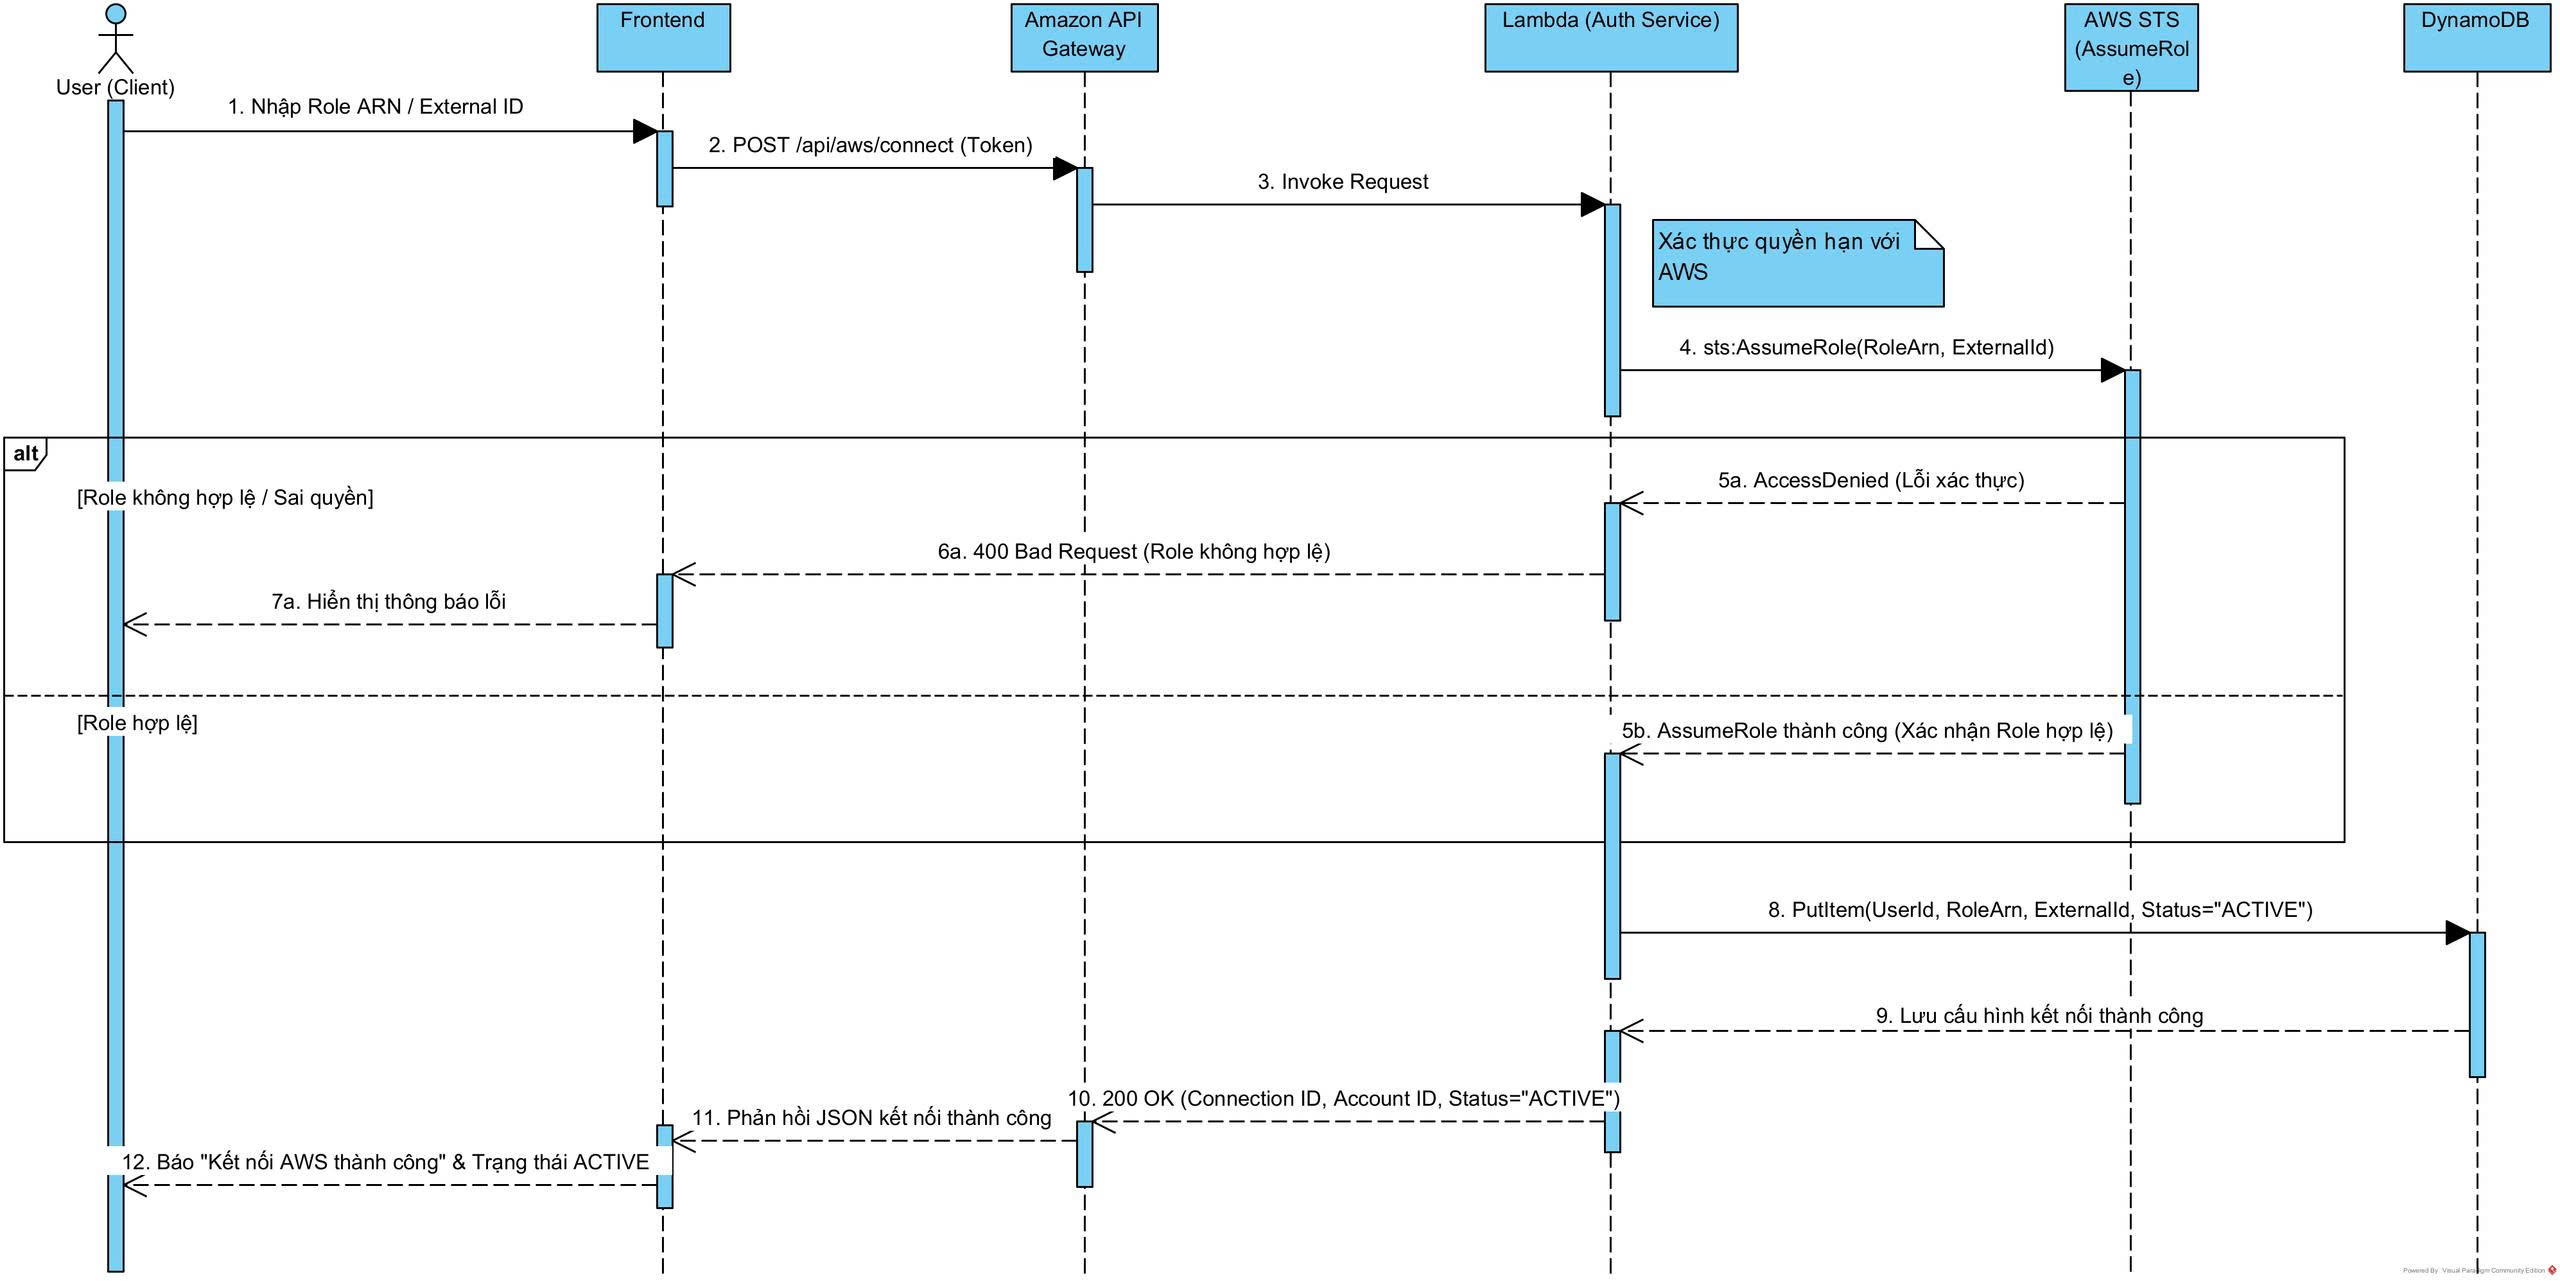
\includegraphics[width=0.78\textwidth]{sequence3.jpg}
  }{
    \IfFileExists{Report progress 2/sequence3.jpg}{
      \includegraphics[width=0.78\textwidth]{Report progress 2/sequence3.jpg}
    }{
      \IfFileExists{Report progress 1/sequence3.jpg}{
        \includegraphics[width=0.78\textwidth]{Report progress 1/sequence3.jpg}
      }{
        \fbox{\parbox[c][5cm][c]{0.88\textwidth}{\centering Sơ đồ tuần tự quy trình kết nối tài khoản AWS}}
      }
    }
  }
  \caption{Sơ đồ tuần tự quy trình kết nối và xác thực tài khoản AWS mục tiêu}
  \label{fig:sequence_connect}
  \end{figure}

  \item \textbf{Quản trị tài nguyên qua Chatbot:} Chatbot Lambda nhận câu lệnh, lấy ngữ cảnh hội thoại từ \texttt{SessionState} và gửi yêu cầu cùng Function Calling Schema đến mô hình LLM. Kết quả được lưu thành hành động chờ xác nhận trong \texttt{PendingAction}. Khi người dùng xác nhận, Chatbot Lambda chuyển ActionID vào SQS cho Dispatcher Lambda; Dispatcher Lambda dùng STS và Boto3 để gọi API của EC2, S3, IAM hoặc Lambda trên AWS của người dùng. Kết quả được lưu vào \texttt{ActionHistory} và gửi về giao diện qua AppSync.

  \begin{figure}[H]
  \centering
  \IfFileExists{sequence1.jpg}{
    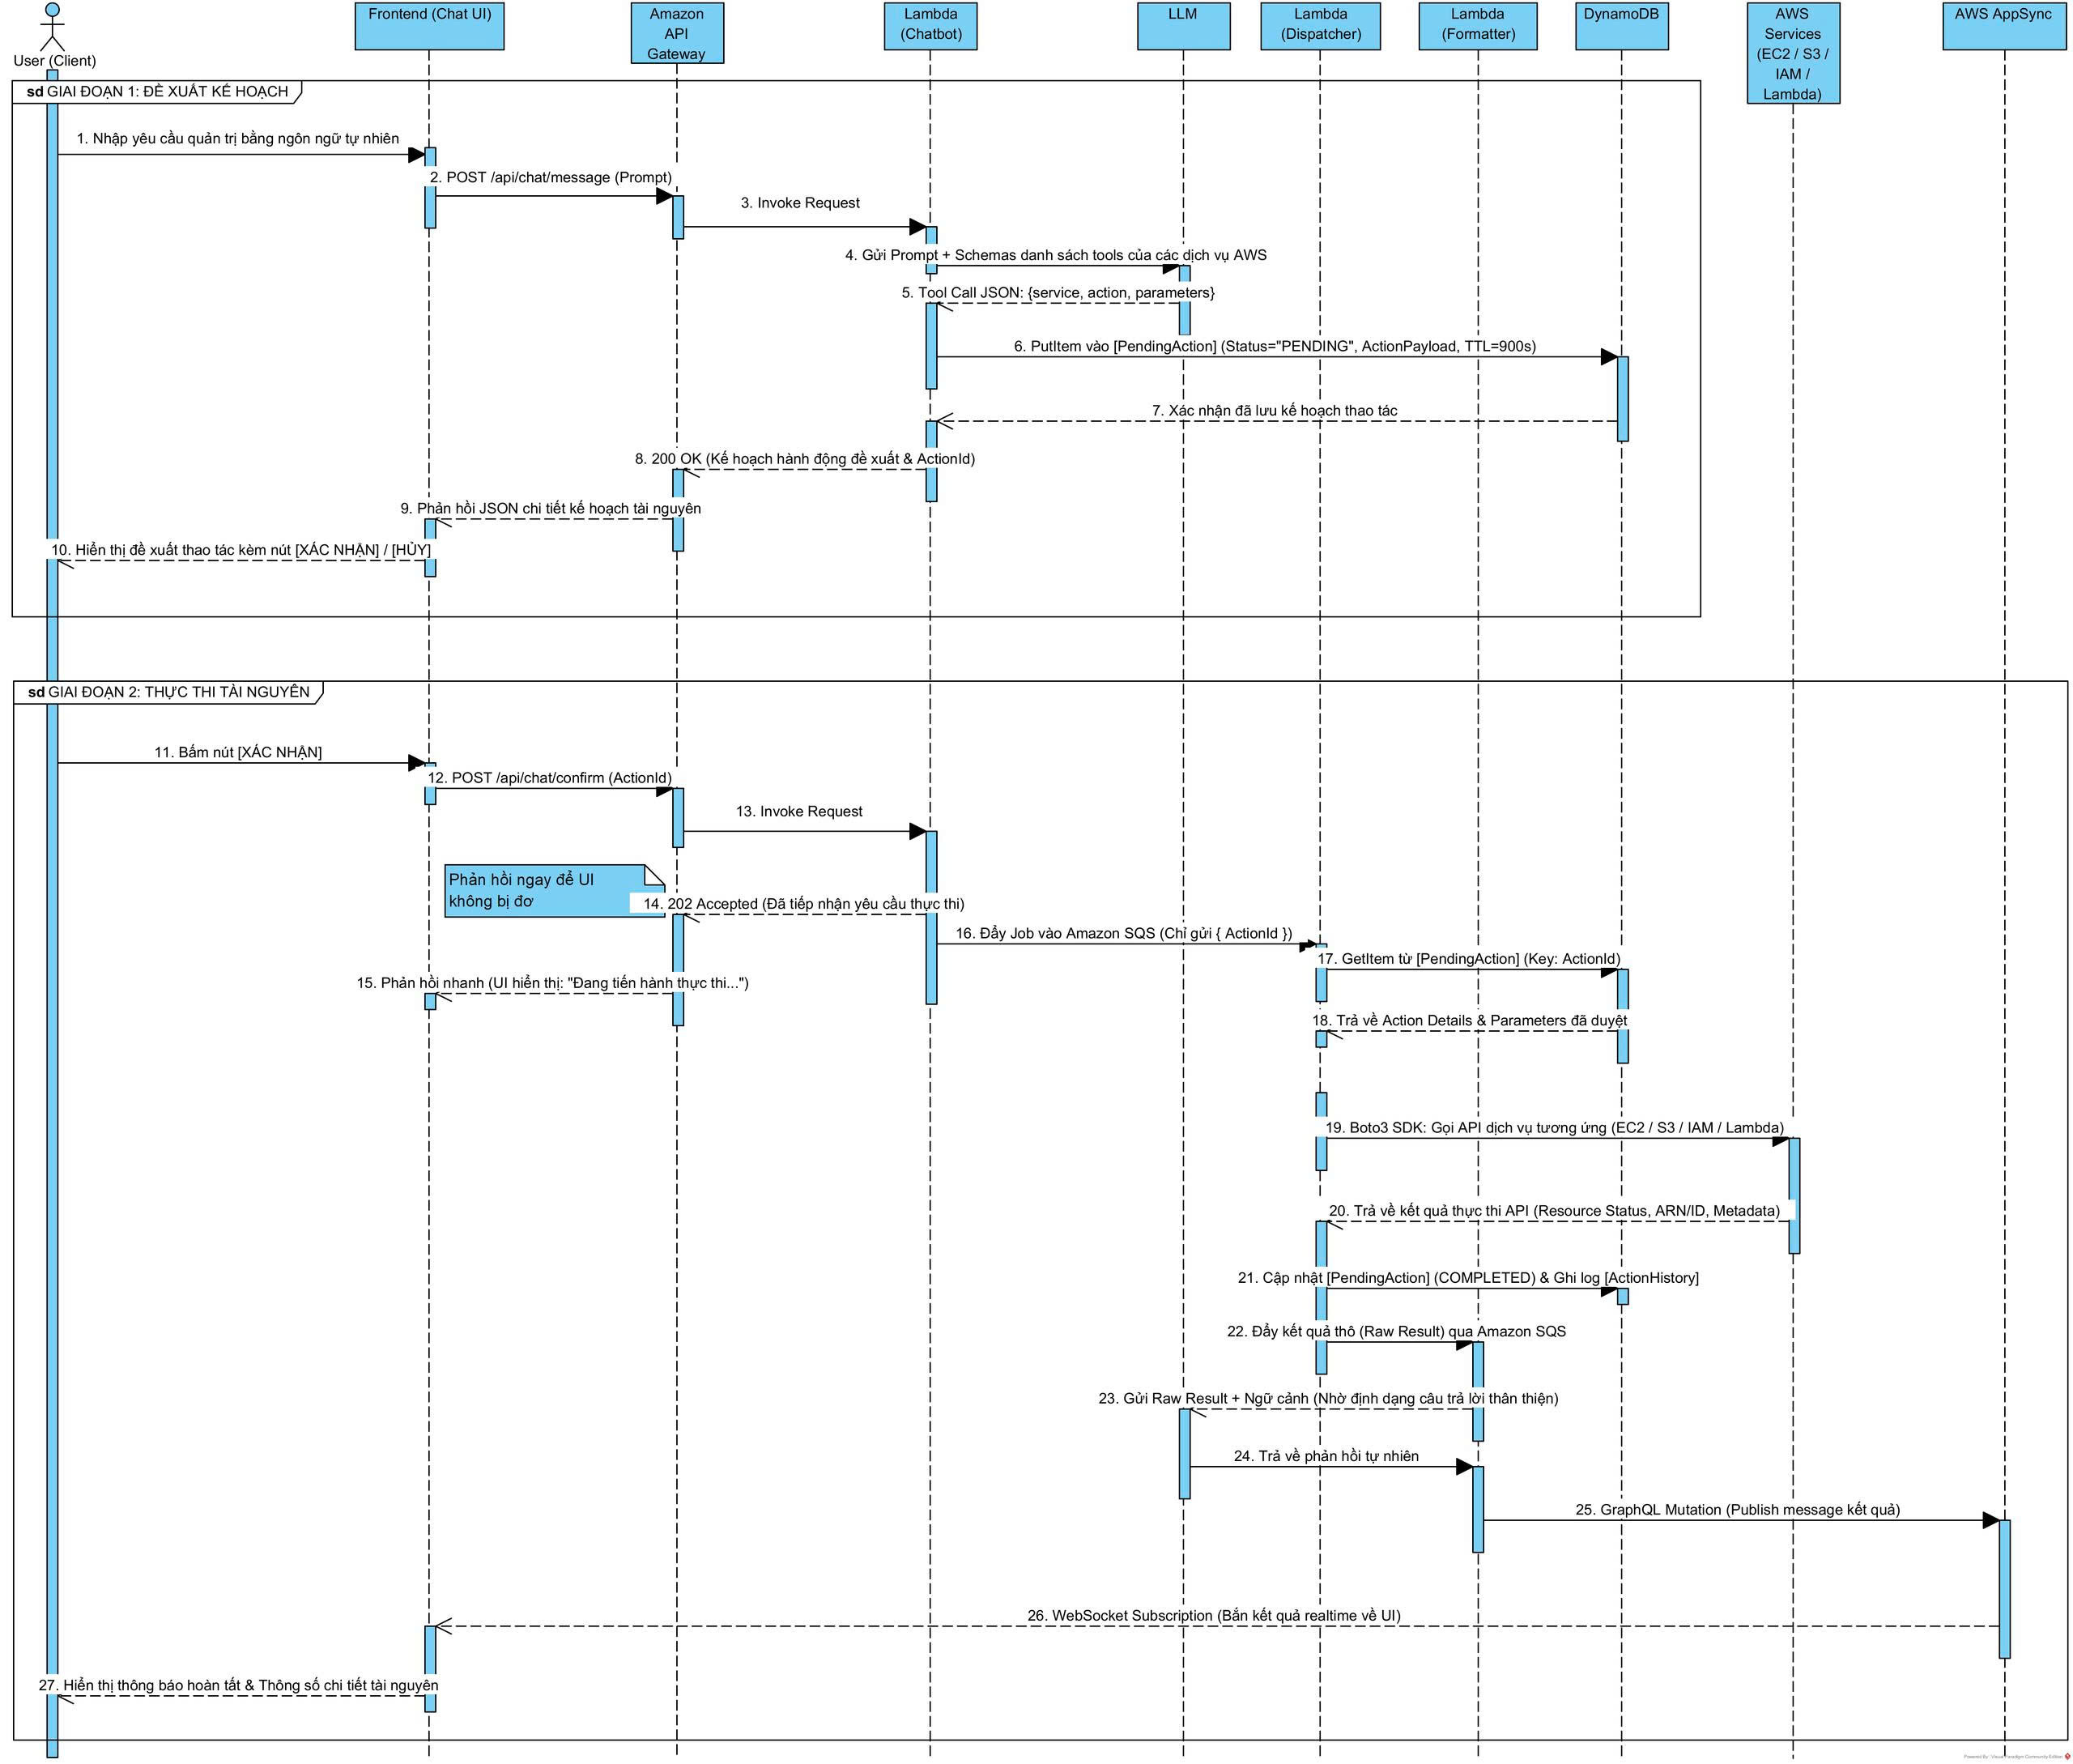
\includegraphics[width=0.8\textwidth]{sequence1.jpg}
  }{
    \IfFileExists{Report progress 2/sequence1.jpg}{
      \includegraphics[width=0.8\textwidth]{Report progress 2/sequence1.jpg}
    }{
      \IfFileExists{Report progress 1/sequence1.jpg}{
        \includegraphics[width=0.8\textwidth]{Report progress 1/sequence1.jpg}
      }{
      }
    }
  }
  \caption{Sơ đồ tuần tự quy trình điều phối và thực thi tác vụ ChatOps}
  \label{fig:sequence_chatops}
  \end{figure}

  \item \textbf{Tra cứu lịch sử thao tác:} History Lambda truy vấn bảng \texttt{ActionHistory} theo người dùng và các điều kiện tra cứu, sau đó trả về thời gian, hành động, tài nguyên đích và trạng thái thực thi để hiển thị trên giao diện.
\end{enumerate}

\subsection{Kiến trúc triển khai của hệ thống}

SatiBot sử dụng các dịch vụ AWS được quản lý để triển khai giao diện, xác thực, xử lý nghiệp vụ và lưu trữ dữ liệu.

\begin{table}[H]
\centering
\caption{Các thành phần và dịch vụ trong kiến trúc triển khai hệ thống SatiBot}
\label{tab:kientruc}
\bangfont
\begin{tabularx}{\linewidth}{@{}>{\raggedright\arraybackslash}p{4.5cm}Y@{}}
\toprule
\textbf{Thành phần / Dịch vụ} & \textbf{Vai trò trong kiến trúc}\\
\midrule
AWS WAF & Tường lửa ứng dụng web, gắn vào CloudFront để lọc request. \\
Amazon Route 53 & Quản lý tên miền (DNS), điều hướng người dùng đến CloudFront. \\
React, Amazon S3 và CloudFront & Cung cấp giao diện ChatOps; S3 lưu các tệp tĩnh và CloudFront phân phối giao diện qua HTTPS.\\
Amazon Cognito & Quản lý đăng ký, đăng nhập và cấp JWT để xác thực người dùng.\\
AWS STS & Cấp quyền truy cập tạm thời (Temporary Credentials). \\
Amazon API Gateway & Tiếp nhận API từ frontend, xác thực JWT và định tuyến yêu cầu chat, xác nhận thao tác hoặc tra cứu lịch sử.\\
AWS Step Functions & Điều phối luồng thực thi sau khi người dùng xác nhận, gồm ChatBot, Dispatcher và Formatter Lambda.\\
AWS Lambda & Thực hiện các nghiệp vụ: Chatbot, Dispatcher, Formatter, Connector và History; Connector đảm nhiệm tạo ExternalId và kiểm tra kết nối AWS.\\
Mô hình LLM & Phân tích câu lệnh tiếng Việt và trả về ý định, tham số theo Function Calling Schema; không trực tiếp gọi API AWS.\\
AWS STS và Boto3 & STS cấp thông tin xác thực tạm thời cho tài khoản đích; Boto3 dùng thông tin này để gọi API tài nguyên.\\
Amazon DynamoDB & Lưu hồ sơ người dùng, kết nối AWS, lịch sử hội thoại, hành động chờ xác nhận và lịch sử thao tác.\\
AWS AppSync & Phát kết quả qua GraphQL Subscriptions để giao diện cập nhật mà không cần polling liên tục.\\
Amazon CloudWatch & Lưu log thực thi và hỗ trợ theo dõi, chẩn đoán lỗi.\\
CI/CD Pipeline (GitHub, CodePipeline, CodeBuild) & Tự động hóa quy trình build, test và deploy. \\
\bottomrule
\end{tabularx}
\end{table}

\subsubsection{Sơ đồ kiến trúc triển khai hệ thống}

\begin{figure}[H]
\centering
\IfFileExists{so_do_kien_truc.jpg}{
  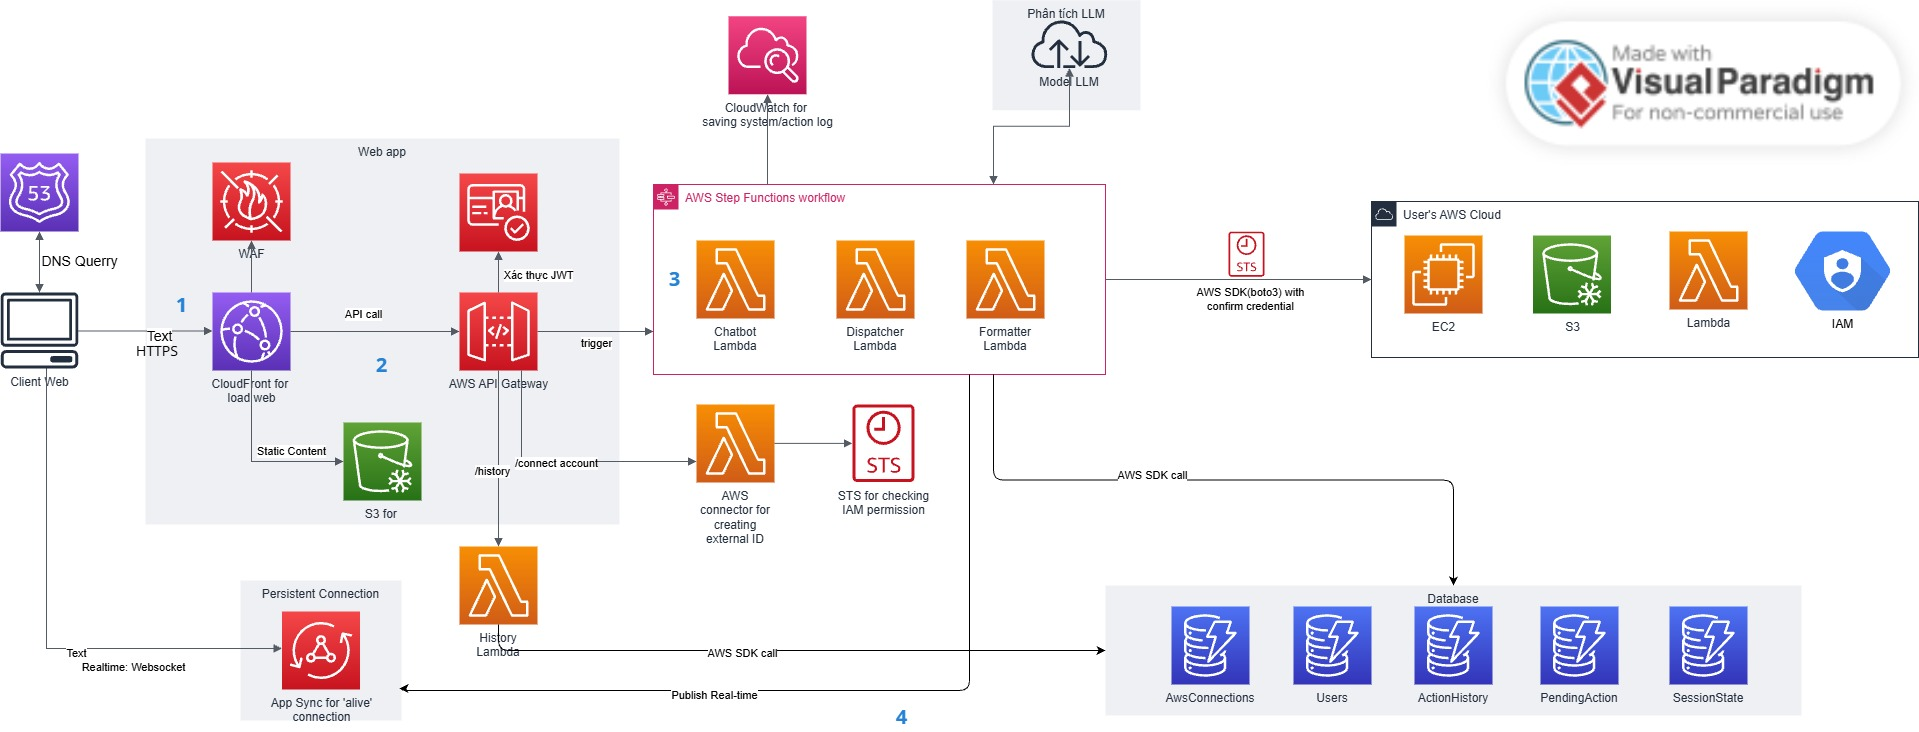
\includegraphics[width=0.82\textwidth]{so_do_kien_truc.jpg}
}{
  \IfFileExists{Report progress 2/so_do_kien_truc.jpg}{
    \includegraphics[width=0.82\textwidth]{Report progress 2/so_do_kien_truc.jpg}
  }{
    \IfFileExists{Report progress 1/so_do_kien_truc.jpg}{
      \includegraphics[width=0.82\textwidth]{Report progress 1/so_do_kien_truc.jpg}
    }{
      \fbox{\parbox[c][6.5cm][c]{0.88\textwidth}{\centering Sơ đồ kiến trúc triển khai tổng thể hệ thống SatiBot}}
    }
  }
}
\caption{Sơ đồ kiến trúc triển khai tổng thể hệ thống SatiBot}
\label{fig:so_do_kien_truc}
\end{figure}


Luồng hoạt động và giao tiếp giữa các thành phần gồm bốn bước:
\begin{enumerate}[itemsep=3pt,topsep=2pt]
  \item \textbf{Tiếp nhận yêu cầu:} Người dùng truy cập ứng dụng web thông qua giao thức HTTPS. Yêu cầu được gửi đến AWS Route53 và trả về IP của CloudFront. Request sẽ đi qua AWS WAF để chặn các request xấu (như chặn SQL Injection, Cross-Site Scripting (XSS), hoặc giới hạn tần suất request để chống DDoS). Sau đó, Amazon CloudFront là nơi phân phối nội dung tĩnh (HTML, CSS, JS) từ Amazon S3. Các yêu cầu API động được CloudFront chuyển tiếp đến Amazon API Gateway. API Gateway sử dụng Amazon Cognito để xác thực JWT Token của người dùng

  \item \textbf{Điều hướng yêu cầu:} Sau khi xác thực thành công, API Gateway kích hoạt dịch vụ tương ứng với yêu cầu của người dùng gồm Lambda for History (truy vấn lịch sử) và AWS core Step Function (Chatbot) .

  \item \textbf{Thực hiện yêu cầu:} Bên trong Step Functions Workflow, các hàm AWS Lambda được triệu gọi tuần tự:
\begin{itemize}
    \item Chatbot Lambda gọi Model LLM để phân tích ý định của người dùng và trích xuất Tool Call. Trạng thái chờ xác nhận được lưu vào bảng \texttt{PendingAction} trong Amazon DynamoDB.
    \item Sau khi người dùng xác nhận, Dispatcher Lambda gọi AWS STS để thực hiện \texttt{AssumeRole} lấy quyền truy cập tạm thời. Sau đó, nó sử dụng AWS SDK (\texttt{Boto3}) để thực thi các lệnh quản lý tài nguyên (như EC2, S3, IAM) trên tài khoản AWS cá nhân của người dùng.
    \item Formatter Lambda gọi lại Model LLM để chuyển đổi kết quả kỹ thuật thô thành ngôn ngữ tự nhiên, đồng thời ghi log hành động vào bảng \texttt{ActionHistory} trong DynamoDB và log hệ thống vào CloudWatch.
\end{itemize}

  \item \textbf{Ghi nhận và trả kết quả:} Formatter Lambda publish thông báo real-time qua AWS AppSync. AppSync duy trì kết nối WebSocket persistent và đẩy thông báo trực tiếp về cho Client/Web
\end{enumerate}

\subsection{Đặc tả chi tiết cần thiết trong giải pháp của dự án}
\subsubsection{Đặc tả cấu hình dịch vụ Bảo mật và Điều hướng}

\textbf{1. Amazon Route 53}
\begin{itemize}[leftmargin=*]
    \item \textbf{Tên miền \& Subdomain:} 
    \begin{itemize}[label=--]
        \item \code{satibot.id.vn} (Giao diện Web).
        \item \code{api.satibot.id.vn} (API Gateway Endpoint).
    \end{itemize}
    
    \item \textbf{Loại bản ghi:} Alias Record (trỏ tới CloudFront Distribution).
    
    \item \textbf{Chứng chỉ SSL/TLS:} AWS Certificate Manager (ACM).
    \begin{itemize}[label=--]
        \item Loại chứng chỉ: Wildcard (\code{*.satibot.id.vn}).
        \item Region cấp phát: \code{us-east-1}.
    \end{itemize}
     
    
    \item \textbf{Chính sách định tuyến:} Failover Routing.
    
    \item \textbf{Cấu hình bản ghi Primary:} Trỏ đến CloudFront của website chính, có S3 origin tại Singapore.
    
    \item \textbf{Cấu hình bản ghi Secondary:} Trỏ đến CloudFront Distribution (Region: \code{us-east-1}; Origin: S3 Bucket chứa tệp \code{error.html}).
    
    \item \textbf{Cấu hình Health Check (áp dụng cho bản ghi Primary):}
    \begin{itemize}[label=--]
        \item Protocol: HTTPS.
        \item Path: \code{/health}.
        \item Request Interval: 10 giây.
        \item Failure Threshold: 3 lần.
    \end{itemize}
    
    \item \textbf{TTL:} 60 giây.
\end{itemize}

\vspace{0.5cm}

\textbf{2. AWS WAF (Web Application Firewall)}
\begin{itemize}[leftmargin=*]
    \item \textbf{Vị trí tích hợp:} Gắn vào CloudFront Distribution.
    
    \item \textbf{Cấu hình Web ACL:}
    \begin{itemize}[label=--]
        \item \textbf{Managed Rule Groups:}
        \begin{itemize}[label=]
            \item \code{AWSManagedRulesCommonRuleSet}: Action = Block.
            \item \code{AWSManagedRulesSQLiRuleSet}: Action = Block.
        \end{itemize}
        
        \item \textbf{Rate-based Rule:}
        \begin{itemize}[label=]
            \item Threshold: 100 requests / 5 phút / 1 IP.
            \item Action: Block.
        \end{itemize}
        
        \item \textbf{IP Sets:} Không cấu hình.
    \end{itemize}
\end{itemize}

\subsubsection{Giao diện và giao thức tương tác giữa các components}
\begin{table}[H]
\centering
\caption{Đặc tả giao diện và giao thức tương tác giữa các components}
\label{tab:inter_service_interfaces}
\begingroup
\renewcommand{\arraystretch}{1.12}
\fontsize{8.5}{11.2}\selectfont
\begin{tabularx}{\linewidth}{@{}>{\raggedright\arraybackslash}p{4.1cm}>{\raggedright\arraybackslash}p{2.35cm}>{\raggedright\arraybackslash}p{3.05cm}Y@{}}
\toprule
\textbf{Nguồn $\rightarrow$ Đích} & \textbf{Giao thức} & \textbf{Xác thực} & \textbf{Dữ liệu trao đổi}\\
\midrule
Web Client $\rightarrow$ CloudFront $\rightarrow$ S3 & HTTPS & TLS & Tệp giao diện tĩnh\\
Web Client $\rightarrow$ API Gateway & HTTPS REST & Cognito JWT & Câu lệnh, session ID, mã hành động\\
API Gateway $\rightarrow$ Chatbot Lambda & Lambda Proxy & IAM & Nội dung chat và thông tin phiên\\
API Gateway $\rightarrow$ Step Functions & StartExecution & IAM Role & User ID và mã hành động đã xác nhận\\
Chatbot Lambda $\leftrightarrow$ LLM & HTTPS API & Theo nhà cung cấp LLM & Prompt, schema công cụ, tham số và kết quả phân tích\\
Step Functions $\rightarrow$ Lambda Tasks & AWS SDK Integration & Step Functions Execution Role & JSON đầu vào/đầu ra từng bước\\
Lambda $\leftrightarrow$ DynamoDB & Boto3 SDK & Lambda Execution Role & GetItem, PutItem, Query, UpdateItem\\
Dispatcher Lambda $\rightarrow$ AWS STS & Boto3 / HTTPS & Lambda Execution Role & AssumeRole với RoleArn và ExternalId\\
Dispatcher $\rightarrow$ Tài khoản AWS đích & Boto3 / HTTPS & Credential tạm thời, SigV4 & Yêu cầu API và kết quả thao tác AWS\\
Formatter Lambda $\rightarrow$ AppSync & GraphQL Mutation / HTTPS & IAM SigV4 & Nội dung kết quả cần phát tới frontend\\
Web Client $\leftrightarrow$ AppSync & GraphQL Subscription / WSS & Cognito User Pool & Sự kiện cập nhật trên khung chat\\
\bottomrule
\end{tabularx}
\endgroup
\end{table}

\subsubsection{Cơ sở dữ liệu hệ thống}
\begin{figure}[H]
\centering
\IfFileExists{so_do_erd.jpg}{
  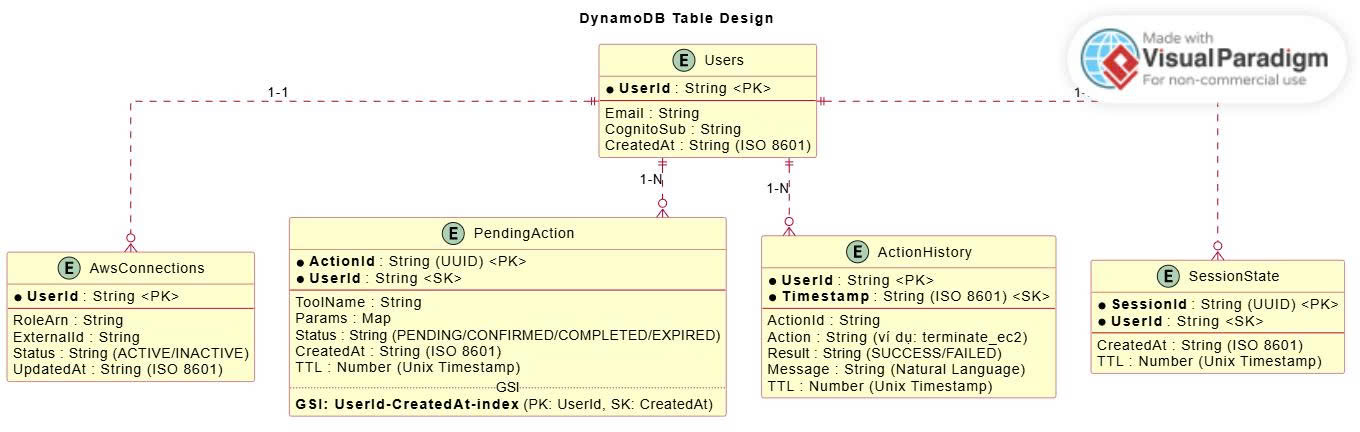
\includegraphics[width=0.9\textwidth]{so_do_erd.jpg}
}{
  \IfFileExists{Report progress 2/so_do_erd.jpg}{
    \includegraphics[width=0.9\textwidth]{Report progress 2/so_do_erd.jpg}
  }{
    \IfFileExists{Report progress 1/so_do_erd.jpg}{
      \includegraphics[width=0.9\textwidth]{Report progress 1/so_do_erd.jpg}
    }{
      \fbox{\parbox[c][6.5cm][c]{0.88\textwidth}{\centering Sơ đồ thực thể liên kết ERD}}
    }
  }
}
\caption{ERD cơ sở dữ liệu hệ thống}
\label{fig:so_do_erd}
\end{figure}



\subsubsection{CI/CD}

Theo thiết kế, quy trình CI/CD của SatiBot bắt đầu khi lập trình viên đẩy mã nguồn lên GitHub và tạo Pull Request. Mã nguồn được các thành viên trong nhóm xem xét, chạy kiểm thử đơn vị và chỉ được hợp nhất vào nhánh \texttt{main} khi đáp ứng yêu cầu. AWS CodeConnections theo dõi nhánh \texttt{main} và kích hoạt AWS CodePipeline khi xuất hiện commit mới. Trong giai đoạn tích hợp liên tục, AWS CodeBuild cài đặt Python cùng các thư viện cần thiết, chạy toàn bộ bộ kiểm thử bằng \texttt{pytest}, sau đó thực hiện \texttt{cdk synth} với hai biến cấu hình \texttt{PRIMARY\_REGION=ap-southeast-1} và \texttt{SECONDARY\_REGION=us-east-1}. Nếu quá trình build hoặc kiểm thử thất bại, pipeline dừng và phát thông báo lỗi; nếu thành công, quy trình chuyển sang bước phê duyệt thủ công. Khi yêu cầu triển khai được chấp thuận, AWS CDK và AWS CloudFormation tiến hành tạo mới hoặc cập nhật các tài nguyên AWS theo cấu hình đã khai báo.

Theo thiết kế, hạ tầng triển khai liên tục được chia thành ba nhóm tài nguyên. Primary Stack tại \texttt{ap-southeast-1} chứa website chính và backend của SatiBot, bao gồm CloudFront, S3, API Gateway, WAF, Lambda, Cognito, IAM và DynamoDB. Các phiên bản Lambda mới được AWS CodeDeploy triển khai theo chiến lược canary; CloudWatch Logs và Alarm theo dõi trạng thái để chuyển toàn bộ lưu lượng sang phiên bản mới khi không có lỗi hoặc tự động rollback khi phát hiện sự cố. Error Page Stack tại \texttt{us-east-1} chỉ sử dụng S3 và CloudFront để cung cấp một trang thông báo lỗi độc lập, không cần đồng bộ dữ liệu ứng dụng với region chính. DNS/Failover Stack sử dụng Amazon Route~53 Health Check và chính sách Failover Routing để theo dõi hệ thống: khi region chính hoạt động bình thường, người dùng được điều hướng đến website tại \texttt{ap-southeast-1}; khi region này gặp sự cố, Route~53 chuyển kết quả phân giải DNS sang trang thông báo lỗi tại \texttt{us-east-1}.

\begin{figure}[H]
\centering
\IfFileExists{cicd.jpg}{
  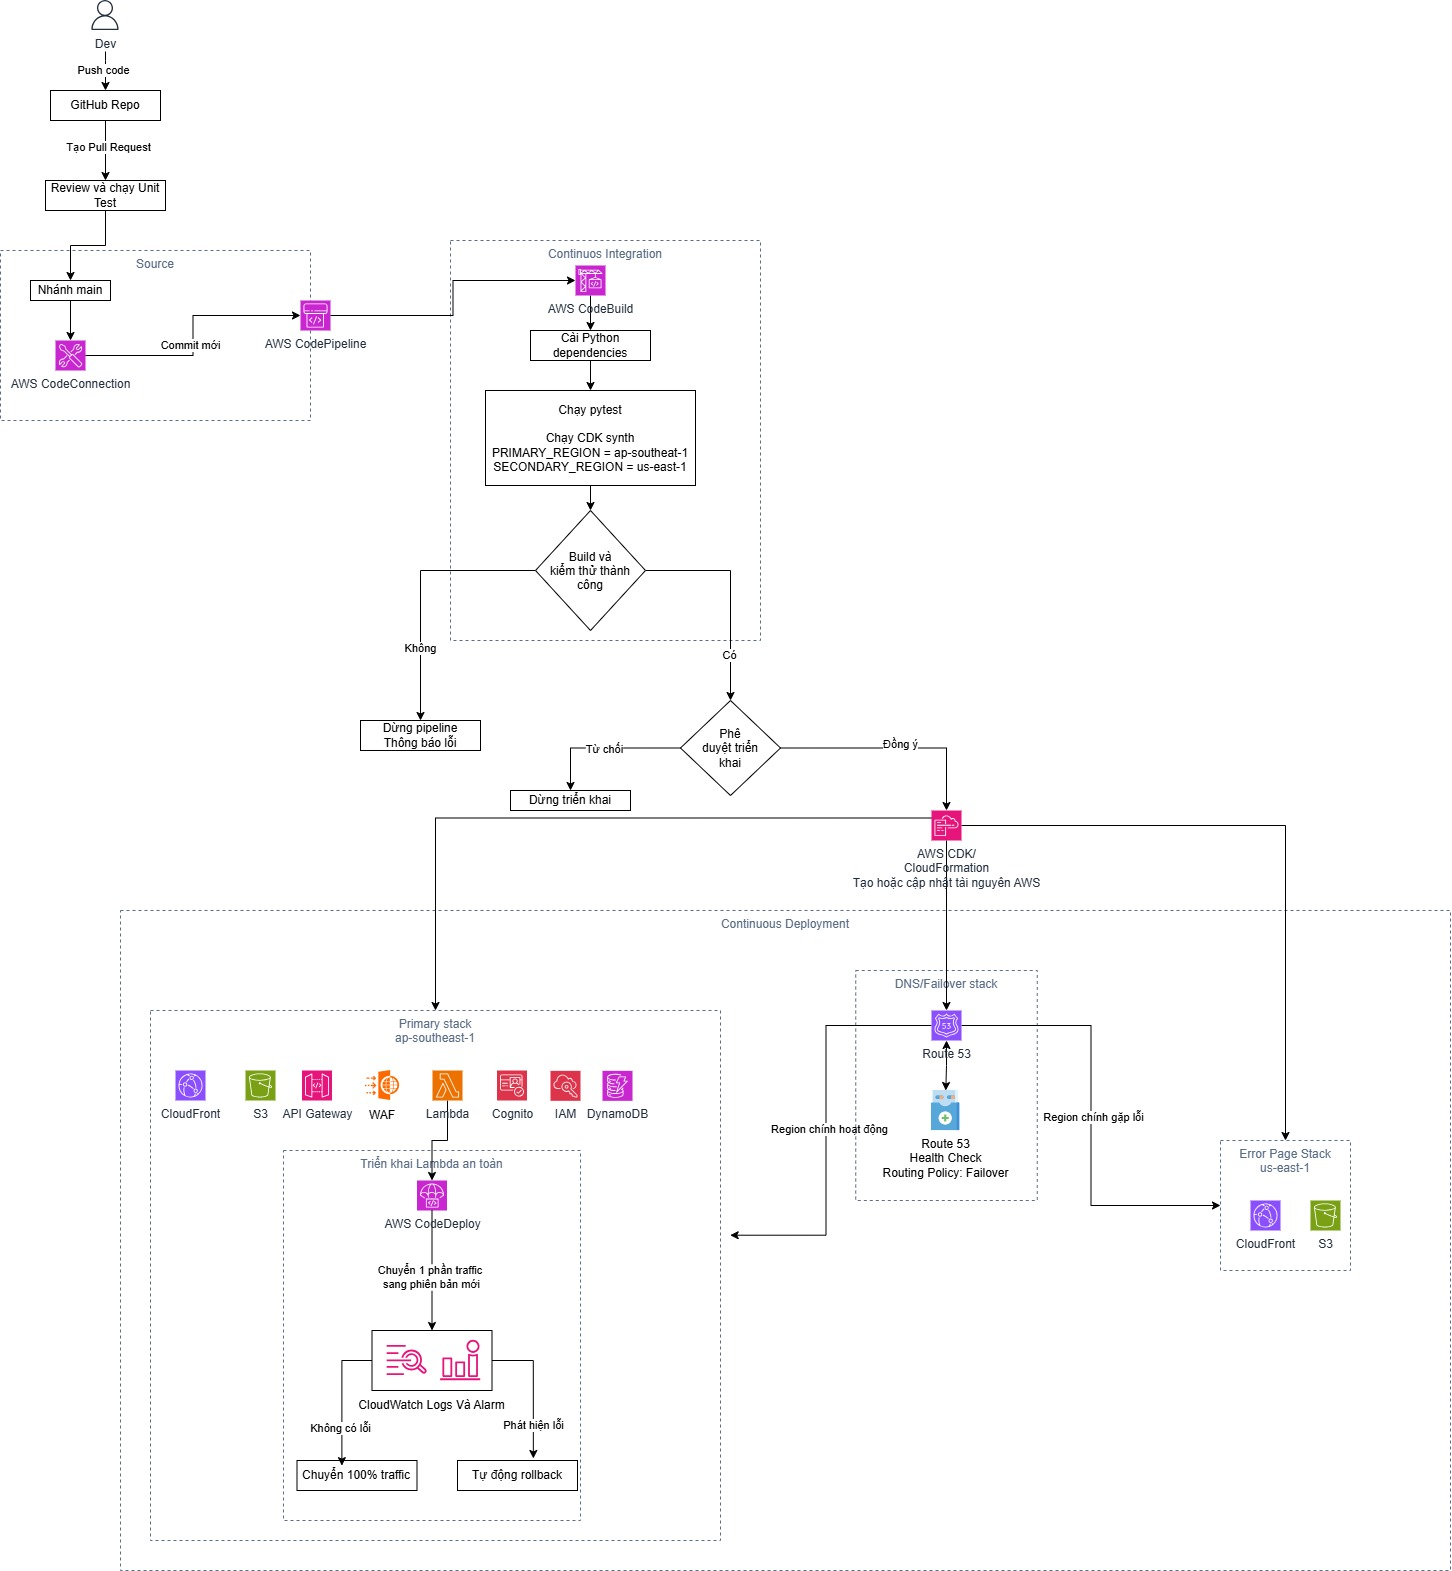
\includegraphics[width=0.95\textwidth,height=0.78\textheight,keepaspectratio]{cicd.jpg}
}{
  \fbox{\parbox[c][7cm][c]{0.92\textwidth}{\centering Sơ đồ quy trình CI/CD của hệ thống SatiBot}}
}
\caption{Quy trình tích hợp, kiểm thử và triển khai liên tục của hệ thống SatiBot}
\label{fig:cicd_pipeline}
\end{figure}

\subsubsection{Phân quyền cho các hàm Lambda}

SatiBot phân quyền theo nhiệm vụ của từng Lambda. Mỗi hàm backend được gắn một IAM role để AWS xác định hàm được phép thực hiện thao tác nào và trên tài nguyên nào. Việc cấp quyền riêng giúp giới hạn tác động khi một hàm gặp lỗi hoặc xử lý sai yêu cầu.

Bảng~\ref{tab:lambda_permissions} trình bày các quyền theo thiết kế cho năm Lambda backend và Lambda ứng dụng trong tài khoản người dùng. Các quyền đọc, ghi được giới hạn vào đúng bảng dữ liệu; quyền đọc khóa Gemini API chỉ được cấp cho những hàm sử dụng mô hình.

\begingroup
\setlength{\tabcolsep}{5pt}
\renewcommand{\arraystretch}{1.17}
\fontsize{10.5}{14}\selectfont
\begin{longtable}{@{}>{\raggedright\arraybackslash}p{2.25cm}>{\raggedright\arraybackslash}p{3.35cm}>{\raggedright\arraybackslash}p{9.05cm}@{}}
\caption{Nhiệm vụ và quyền IAM của các Lambda}\label{tab:lambda_permissions}\\
\toprule
\textbf{Lambda} & \textbf{Nhiệm vụ} & \textbf{IAM Action cần cấp và nơi sử dụng}\\
\midrule
\endfirsthead
\toprule
\textbf{Lambda} & \textbf{Nhiệm vụ} & \textbf{IAM Action cần cấp và nơi sử dụng}\\
\midrule
\endhead
\endfoot
\bottomrule
\endlastfoot
Chatbot & Xử lý câu chat; lưu phiên và hành động chờ xác nhận. &
\path{dynamodb:GetItem}: đọc SessionState, PendingAction và AwsConnections.\par
\path{dynamodb:PutItem}, \path{dynamodb:UpdateItem}: ghi SessionState và PendingAction.\par
\path{secretsmanager:GetSecretValue}: đọc khóa Gemini API.\\
\midrule
Dispatcher & Thực thi hành động đã duyệt trên tài khoản AWS đích. &
\path{dynamodb:GetItem}: đọc PendingAction và AwsConnections.\par
\path{dynamodb:UpdateItem}: cập nhật PendingAction.\par
\path{sts:AssumeRole}: nhận quyền tạm thời từ role trong tài khoản đích.\\
\midrule
Formatter & Tạo lời đáp; lưu và gửi kết quả. &
\path{dynamodb:PutItem}, \path{dynamodb:UpdateItem}: ghi ActionHistory.\par
\path{appsync:GraphQL}: phát kết quả qua AppSync.\par
\path{secretsmanager:GetSecretValue}: đọc khóa Gemini API.\\
\midrule
Connector & Tạo ExternalId; lưu và kiểm tra kết nối AWS. &
\path{dynamodb:GetItem}, \path{dynamodb:PutItem}, \path{dynamodb:UpdateItem}: quản lý AwsConnections.\par
\path{sts:AssumeRole}: kiểm tra role người dùng cung cấp.\\
\midrule
History & Liệt kê và xem chi tiết lịch sử. &
\path{dynamodb:Query}: liệt kê bản ghi trong ActionHistory.\par
\path{dynamodb:GetItem}: đọc một bản ghi trong ActionHistory.\\
\midrule
Lambda của người dùng & Chạy mã ứng dụng trong tài khoản AWS đích. &
Quyền phụ thuộc mã ứng dụng; ví dụ \path{s3:GetObject} khi hàm cần đọc tệp S3. Quyền quản lý hàm, như \path{lambda:InvokeFunction} hoặc \path{lambda:UpdateFunctionConfiguration}, nằm trong role đích mà Dispatcher đảm nhận.\\
\end{longtable}
\endgroup

Để thao tác trên tài khoản AWS của người dùng, Connector và Dispatcher sử dụng role do chủ tài khoản cho phép SatiBot truy cập. Connector kiểm tra kết nối; Dispatcher nhận quyền tạm thời qua STS để thực hiện các thao tác được role đó cho phép. Lambda ứng dụng của người dùng có quyền chạy riêng, tùy theo mã ứng dụng. Các Lambda ghi log được cấp thêm quyền ghi CloudWatch Logs để theo dõi lỗi.

\subsubsection{Tích hợp LLM qua Gemini API}
\label{sec:llm_integration}

Hệ thống sử dụng mô hình Gemini của Google qua Gemini API. Tại Chatbot Lambda, mô hình chuyển câu chat tiếng Việt thành yêu cầu gọi hàm quản trị AWS; tại Formatter Lambda, mô hình diễn giải kết quả thực thi. Việc thao tác tài nguyên do Dispatcher thực hiện bằng Boto3 theo luồng ở Hình~\ref{fig:sequence_chatops}.


\begin{figure}[H]
\centering
\begin{tikzpicture}[x=1cm,y=1cm,
box/.style={draw,rounded corners,align=center,text width=3.6cm,minimum height=1cm,font=\small},
lab/.style={font=\footnotesize,align=center,fill=white,inner sep=2pt}]
\node[box] (chat) at (0,0) {Chatbot Lambda\\Chuẩn bị yêu cầu};
\node[box] (llm) at (8,0) {Gemini API\\Chọn hàm và tham số};
\node[box] (check) at (0,-2.5) {Chatbot Lambda\\Kiểm tra, yêu cầu xác nhận};
\node[box] (dispatch) at (8,-2.5) {Dispatcher Lambda\\Boto3 gọi AWS};
\draw[->,thick] (chat.north east) -- ++(0,.6) -| node[lab,pos=.25,above] {Câu chat, ngữ cảnh, danh sách hàm} (llm.north);
\draw[->,thick] (llm.west) -- node[lab,above] {Tên hàm và tham số} (chat.east);
\draw[->,thick] (chat) -- (check);
\draw[->,thick] (check) -- node[lab,above] {Hành động đủ điều kiện\\thực thi} (dispatch);
\end{tikzpicture}
\caption{Tích hợp Gemini API với các Lambda xử lý yêu cầu}
\label{fig:llm_integration}
\end{figure}

Backend gọi Gemini API bằng HTTP POST qua HTTPS, sử dụng endpoint Chat Completions do Google cung cấp. Nội dung request và response có định dạng JSON; khóa API được gửi trong header Authorization. Endpoint và mã model là cấu hình backend, model cần hỗ trợ Function Calling. Theo phương án triển khai, khóa API được lưu trong Secrets Manager và chỉ các Lambda cần gọi LLM được quyền đọc.

\begin{table}[H]
\centering
\caption{Dữ liệu trao đổi giữa Chatbot Lambda và Gemini API}
\label{tab:llm_exchange}
\fontsize{11}{14}\selectfont
\begin{tabularx}{\linewidth}{@{}>{\raggedright\arraybackslash}p{2.4cm}>{\raggedright\arraybackslash}p{3.2cm}Y@{}}
\toprule
\textbf{Chiều trao đổi} & \textbf{Trường dữ liệu} & \textbf{Nội dung}\\
\midrule
Gửi tới Gemini & \texttt{model} & Mã mô hình Gemini được cấu hình cho hệ thống.\\
 & \texttt{messages} & Chỉ dẫn hệ thống, câu chat hiện tại và ngữ cảnh hội thoại cần thiết.\\
 & \texttt{tools} & Danh sách hàm được phép gọi: tên, mô tả và JSON Schema quy định tham số.\\
 & \texttt{tool\_choice} & Giá trị \texttt{auto}: cho phép mô hình trả lời hoặc đề xuất gọi hàm theo yêu cầu.\\
\midrule
Nhận từ Gemini & \texttt{content} & Nội dung trả lời hoặc câu hỏi bổ sung khi chưa đủ thông tin.\\
 & \texttt{tool\_calls} & Danh sách lời gọi hàm; mỗi lời gọi có tên hàm và các tham số.\\
\bottomrule
\end{tabularx}
\end{table}

Danh sách hàm được khai báo trước cho bốn module EC2, S3, IAM và Lambda. Mỗi khai báo mô tả một thao tác và các tham số bắt buộc, kiểu dữ liệu, giá trị cho phép. Khi nhận \texttt{tool\_calls}, Chatbot kiểm tra tên hàm và tham số theo khai báo, rồi ánh xạ sang thao tác tương ứng của Dispatcher.

Formatter gửi kết quả AWS cho LLM để tạo lời đáp dễ đọc, không cần cung cấp danh sách hàm quản trị. Trạng thái thực thi, định danh tài nguyên và số liệu được lấy từ kết quả AWS; nội dung do LLM diễn giải không thay thế các dữ liệu này. Nếu bước diễn giải lỗi, Formatter trả kết quả theo mẫu có sẵn.

Mỗi lần gọi LLM có thời gian chờ và số lần thử lại giới hạn. Phản hồi sai cấu trúc không được chuyển sang thực thi. Ngữ cảnh hội thoại được giới hạn số lượt và dung lượng; credential AWS không được gửi tới mô hình. Lỗi kết nối hoặc lỗi tạo lời đáp không làm chạy lại thao tác thay đổi tài nguyên đã thực hiện.


\subsubsection{Endpoint tiếp nhận hội thoại và trích xuất ý định (POST /chat)}

\textbf{1. Thông tin chung:}
\begin{itemize}
    \item \textbf{Đường dẫn (Path):} \texttt{/chat} (hoặc \texttt{/api/chat} trên giao diện Web Client).
    \item \textbf{Phương thức HTTP:} \texttt{POST}.
    \item \textbf{Cơ chế xác thực:} Bearer JWT Token thông qua HTTP Header \texttt{Authorization: Bearer <Token>}. Amazon API Gateway sử dụng Cognito User Pool Authorizer để giải mã và kiểm tra tính hợp lệ của token trước khi kích hoạt hàm xử lý phía sau.
    \item \textbf{Thành phần tiếp nhận:} Amazon API Gateway $\rightarrow$ Chatbot Lambda (tích hợp mô hình ngôn ngữ lớn LLM với cơ chế Function Calling).
\end{itemize}

\textbf{2. Dữ liệu trao đổi minh họa (Kịch bản khởi tạo máy chủ ảo EC2):}

Mẫu JSON Request gửi từ Web Client khi người dùng gửi câu lệnh khởi tạo máy chủ EC2 bằng ngôn ngữ tự nhiên tiếng Việt:

\begin{verbatim}
{
  "message": "Tạo cho tôi một máy chủ EC2 Ubuntu có tên 'web-demo'",
  "history": [
    {
      "role": "user",
      "content": "Xin chào SatiBot"
    },
    {
      "role": "assistant",
      "content": "Xin chào! Tôi là SatiBot."
    }
  ],
  "region": "ap-southeast-1"
}
\end{verbatim}

Mẫu JSON Response trả về từ hệ thống. Do thao tác \texttt{create\_instance} là hành động làm thay đổi tài nguyên hạ tầng và phát sinh chi phí, hệ thống trả về mã trạng thái \texttt{CONFIRMATION\_REQUIRED} kèm mã giao dịch \texttt{action\_id} để yêu cầu xác nhận:

\begin{verbatim}
{
  "status": "CONFIRMATION_REQUIRED",
  "type": "action_confirmation",
  "action_id": "act_8f3a9e1b2c4d",
  "service": "ec2",
  "tool_name": "create_instance",
  "parameters": {
    "instance_name": "web-demo",
    "os_type": "ubuntu",
    "instance_type": "t3.micro"
  },
  "message": "Xác nhận tạo máy chủ EC2 web-demo?"
}
\end{verbatim}

\textbf{3. Bảng giải thích chi tiết các trường dữ liệu:}

\begin{table}[H]
\centering
\caption{Mô tả các trường trong Request Body của Endpoint \texttt{POST /chat}}
\label{tab:chat_request}
\begingroup
\renewcommand{\arraystretch}{1.12}
\fontsize{10}{13}\selectfont
\begin{tabularx}{\linewidth}{@{}>{\raggedright\arraybackslash}p{2.5cm}>{\raggedright\arraybackslash}p{2.3cm}>{\centering\arraybackslash}p{1.8cm}Y@{}}
\toprule
\textbf{Tên trường} & \textbf{Kiểu dữ liệu} & \textbf{Bắt buộc} & \textbf{Mô tả ý nghĩa và nguồn gốc dữ liệu} \\
\midrule
\texttt{message} & String & Có & Nội dung câu lệnh bằng ngôn ngữ tự nhiên tiếng Việt của người dùng gửi từ giao diện. \\
\texttt{history} & Array[Object] & Không & Lịch sử hội thoại nhiều lượt gồm các cặp \texttt{role} và \texttt{content}, đồng bộ từ bảng \texttt{SessionState} trong DynamoDB. \\
\texttt{region} & String & Không & Khu vực AWS mục tiêu thực hiện tác vụ (mặc định: \texttt{ap-southeast-1}). \\
\texttt{session\_id} & String & Không & Mã phiên hội thoại; giao diện dùng để ghép yêu cầu với lịch sử. Credential AWS không được gửi trực tiếp từ website. \\
\bottomrule
\end{tabularx}
\endgroup
\end{table}

\begin{table}[H]
\centering
\caption{Mô tả các trường trong Response Body của Endpoint \texttt{POST /chat}}
\label{tab:chat_response}
\begingroup
\renewcommand{\arraystretch}{1.12}
\fontsize{10}{13}\selectfont
\begin{tabularx}{\linewidth}{@{}>{\raggedright\arraybackslash}p{2.8cm}>{\raggedright\arraybackslash}p{2.2cm}>{\centering\arraybackslash}p{1.8cm}Y@{}}
\toprule
\textbf{Tên trường} & \textbf{Kiểu dữ liệu} & \textbf{Bắt buộc} & \textbf{Mô tả ý nghĩa và nguồn gốc dữ liệu} \\
\midrule
\texttt{status} & String & Có & Trạng thái phản hồi của hệ thống (\texttt{CONFIRMATION\_REQUIRED} khi cần duyệt, hoặc \texttt{SUCCESS} khi chỉ truy vấn dữ liệu). \\
\texttt{type} & String & Có & Loại phản hồi định hướng hiển thị phía Client (\texttt{action\_confirmation} hoặc \texttt{chat\_reply}). \\
\texttt{action\_id} & String & Có & Mã định danh duy nhất cho hành động chờ duyệt, được lưu làm Partition Key trong bảng \texttt{PendingAction} với thời gian TTL 15 phút. \\
\texttt{service} & String & Có & Dịch vụ AWS mục tiêu (ví dụ: \texttt{ec2}, \texttt{s3}, \texttt{lambda}, \texttt{iam}) do LLM Function Calling trích xuất. \\
\texttt{tool\_name} & String & Có & Tên hành động kỹ thuật được trích xuất (ví dụ: \texttt{create\_instance}, \texttt{manage\_power}). \\
\texttt{parameters} & Object & Có & Cấu trúc tham số kỹ thuật chi tiết trích xuất từ câu lệnh tự nhiên của người dùng. \\
\texttt{message} & String & Có & Lời nhắn tiếng Việt thân thiện gửi người dùng để thông báo hoặc yêu cầu xác nhận an toàn. \\
\bottomrule
\end{tabularx}
\endgroup
\end{table}

\subsubsection{Endpoint xác nhận và thực thi tài nguyên (POST /confirm)}

\textbf{1. Thông tin chung:}
\begin{itemize}
    \item \textbf{Đường dẫn (Path):} \texttt{/confirm} (hoặc gửi tới \texttt{/chat} với tham số \texttt{confirmed: true}).
    \item \textbf{Phương thức HTTP:} \texttt{POST}.
    \item \textbf{Cơ chế xác thực:} JWT Cognito trong header \texttt{Authorization}.
    \item \textbf{Thành phần tiếp nhận:} Amazon API Gateway $\rightarrow$ Chatbot Lambda / Step Functions $\rightarrow$ Dispatcher Lambda $\rightarrow$ EC2 Service (\texttt{boto3.client('ec2')}) $\rightarrow$ Amazon DynamoDB (\texttt{ActionHistory}).
\end{itemize}

\textbf{2. Dữ liệu trao đổi minh họa (Kịch bản người dùng chấp thuận tạo máy ảo):}

Mẫu JSON Request gửi từ Web Client khi người dùng nhấn nút ``Xác nhận thực thi'' trên giao diện:

\begin{verbatim}
{
  "confirmed": true,
  "action_id": "act_8f3a9e1b2c4d",
  "service": "ec2",
  "tool_name": "create_instance",
  "parameters": {
    "instance_name": "web-demo",
    "os_type": "ubuntu",
    "instance_type": "t3.micro"
  },
  "region": "ap-southeast-1"
}
\end{verbatim}

Mẫu JSON Response minh họa khi Dispatcher Lambda và module EC2 Service thực thi thành công trong khu vực Singapore:

\begin{verbatim}
{
  "status": "SUCCESS",
  "type": "action_executed",
  "service": "ec2",
  "tool_name": "create_instance",
  "message": "Đã gửi yêu cầu tạo máy chủ web-demo.",
  "data": {
    "instance_id": "i-015aad95042137744",
    "instance_name": "web-demo",
    "state": "pending",
    "instance_type": "t3.micro",
    "image_id": "ami-0af9110f0ec0820e2"
  }
}
\end{verbatim}

\textbf{3. Bảng giải thích chi tiết các trường dữ liệu:}

\begin{table}[H]
\centering
\caption{Mô tả các trường trong Request Body của Endpoint \texttt{POST /confirm}}
\label{tab:confirm_request}
\begingroup
\renewcommand{\arraystretch}{1.12}
\fontsize{10}{13}\selectfont
\begin{tabularx}{\linewidth}{@{}>{\raggedright\arraybackslash}p{2.5cm}>{\raggedright\arraybackslash}p{2.3cm}>{\centering\arraybackslash}p{1.8cm}Y@{}}
\toprule
\textbf{Tên trường} & \textbf{Kiểu dữ liệu} & \textbf{Bắt buộc} & \textbf{Mô tả ý nghĩa và nguồn gốc dữ liệu} \\
\midrule
\texttt{confirmed} & Boolean & Có & Cờ xác nhận mang giá trị \texttt{true}, khẳng định người dùng đã trực tiếp phê duyệt hành động. \\
\texttt{action\_id} & String & Có & Mã hành động tương ứng đã tạo ở bước \texttt{/chat}, dùng để đối soát trạng thái trong bảng \texttt{PendingAction}. \\
\texttt{service} & String & Có & Dịch vụ AWS đích cần điều phối thực thi (\texttt{ec2}, \texttt{s3}, \texttt{lambda}, \texttt{iam}). \\
\texttt{tool\_name} & String & Có & Tên hành động kỹ thuật cần thực thi (\texttt{create\_instance}, v.v.). \\
\texttt{parameters} & Object & Có & Tập tham số kỹ thuật đã qua rà soát của người quản trị. \\
\texttt{region} & String & Không & Khu vực thực thi lệnh trên đám mây AWS (mặc định: \texttt{ap-southeast-1}). \\
\bottomrule
\end{tabularx}
\endgroup
\end{table}

\begin{table}[H]
\centering
\caption{Mô tả các trường trong Response Body của Endpoint \texttt{POST /confirm}}
\label{tab:confirm_response}
\begingroup
\renewcommand{\arraystretch}{1.12}
\fontsize{10}{13}\selectfont
\begin{tabularx}{\linewidth}{@{}>{\raggedright\arraybackslash}p{3.2cm}>{\raggedright\arraybackslash}p{2.0cm}>{\centering\arraybackslash}p{1.8cm}Y@{}}
\toprule
\textbf{Tên trường} & \textbf{Kiểu dữ liệu} & \textbf{Bắt buộc} & \textbf{Mô tả ý nghĩa và nguồn gốc dữ liệu} \\
\midrule
\texttt{status} & String & Có & Kết quả xử lý hạ tầng tổng thể (\texttt{SUCCESS} hoặc \texttt{ERROR}). \\
\texttt{type} & String & Có & Phân loại giao diện (\texttt{action\_executed}) để Web Client cập nhật trạng thái thẻ hiển thị sang hoàn tất. \\
\texttt{service} & String & Có & Tên dịch vụ AWS đã thực thi hoàn tất (\texttt{ec2}). \\
\texttt{tool\_name} & String & Có & Tên công cụ kỹ thuật đã chạy (\texttt{create\_instance}). \\
\texttt{message} & String & Có & Thông báo tổng kết kỹ thuật bằng tiếng Việt kèm mã ID và trạng thái máy ảo. \\
\texttt{data} & Object & Có & Đối tượng chứa dữ liệu chi tiết trả về từ Boto3 SDK gồm: \texttt{instance\_id}, \texttt{instance\_name}, \texttt{state} (trạng thái \texttt{pending} non-blocking), \texttt{instance\_type} và mã \texttt{image\_id} chính thức của hệ điều hành. \\
\bottomrule
\end{tabularx}
\endgroup
\end{table}



\clearpage
\section{KẾT QUẢ THỰC HIỆN}

Chương này trình bày quy trình triển khai hoàn chỉnh hệ thống SatiBot lên môi trường điện toán đám mây AWS tại tên miền \url{https://satibot.id.vn/} cùng các kết quả kiểm thử, nghiệm thu cho quy trình CI/CD, bảo mật biên và chuyển đổi dự phòng, các kịch bản quản trị dịch vụ AWS qua giao diện ChatOps và đánh giá hiệu năng vận hành thực tế.

\subsection{Các bước triển khai hệ thống thực tế (Deployment Steps)}

Hệ thống được mô hình hóa hoàn toàn theo Infrastructure as Code (IaC) bằng AWS CDK và triển khai theo thứ tự phụ thuộc Multi-Region giữa region chính Singapore (\code{ap-southeast-1}) và region dự phòng Bắc Virginia (\code{us-east-1}):

\begin{enumerate}[itemsep=3pt,topsep=2pt]
  \item \textbf{Khởi tạo tầng dữ liệu và phân quyền:} Thực thi \code{cdk bootstrap} trên cả hai region; triển khai 5 bảng DynamoDB (user, AWS connections, session state, pending action, action history) và các IAM Role theo nguyên tắc Least Privilege tách riêng cho từng hàm Lambda và dịch vụ CodeDeploy.
  \item \textbf{Thiết lập bảo vệ biên và trang fallback Multi-Region:} Triển khai Web ACL của AWS WAF, cấp chứng chỉ SSL/TLS bao phủ tên miền \code{satibot.id.vn} và tạo S3 bucket riêng tư chứa trang fallback tĩnh (Maintenance Page) tại \code{us-east-1}.
  \item \textbf{Đóng gói và triển khai Backend Serverless:} Chạy Unit Test, đóng gói 5 hàm Lambda nghiệp vụ (\code{Chatbot}, \code{Dispatcher}, \code{Formatter}, \code{Connector}, \code{History}) cùng Workflow Step Functions, cấu hình alias \code{live} gắn CodeDeploy Canary và 5 CloudWatch Alarm.
  \item \textbf{Kết nối lớp xác thực và giao tiếp real-time:} Triển khai Amazon Cognito (OAuth2/PKCE), API Gateway REST API tích hợp trực tiếp tới alias \code{live}, và AWS AppSync GraphQL/WebSocket để đẩy kết quả từ backend về trình duyệt ngay khi hoàn tất.
  \item \textbf{Deploy giao diện, gắn tên miền và kích hoạt CI/CD:} Đưa ứng dụng React lên S3 qua CloudFront CDN gắn Origin Group dự phòng; cấu hình Route~53 DNS; đồng thời nối GitHub App tới AWS CodePipeline để tự động hóa toàn bộ quy trình CI/CD.
\end{enumerate}

Bảng~\ref{tab:deployed_architecture} tổng hợp các nhóm dịch vụ thuộc 12 CloudFormation stack đã triển khai.

\begingroup
\setlength{\tabcolsep}{6pt}
\renewcommand{\arraystretch}{1.18}
\fontsize{10.5}{14}\selectfont
\begin{longtable}{@{}>{\raggedright\arraybackslash}p{3.6cm}>{\raggedright\arraybackslash}p{4.8cm}>{\raggedright\arraybackslash}p{\dimexpr\linewidth-8.4cm-4\tabcolsep\relax}@{}}
\caption{Kiến trúc triển khai thực tế của hệ thống SatiBot trên hai region AWS}\label{tab:deployed_architecture}\\
\toprule
\textbf{Tầng kiến trúc} & \textbf{Dịch vụ AWS (Region)} & \textbf{Vai trò trong hệ thống vận hành}\\
\midrule
\endfirsthead
\endhead
\endfoot
\bottomrule
\endlastfoot
Giao diện \& Bảo vệ biên & S3, CloudFront, Route~53, ACM, AWS WAF (\code{ap-southeast-1} \& \code{us-east-1}) & Phân phối ứng dụng qua HTTPS, định tuyến DNS, chặn XSS/SQLi/Rate-limit và trả về trang fallback khi origin chính lỗi.\\
Xác thực \& Kết nối API & Amazon Cognito, API Gateway, AWS AppSync (\code{ap-southeast-1}) & Xác thực người dùng bằng JWT, tiếp nhận request hội thoại/xác nhận và đẩy kết quả real-time về trình duyệt qua WebSocket.\\
Xử lý Serverless \& Điều phối & 5 Lambda nghiệp vụ, Lambda \code{HealthCheck}, Step Functions (\code{ap-southeast-1}) & Phân tích ý định qua Gemini API, thực thi thao tác trên tài khoản AWS đích bằng STS \code{AssumeRole} và định dạng phản hồi.\\
Dữ liệu \& Bảo mật nội bộ & 5 bảng DynamoDB, IAM, Secrets Manager (\code{ap-southeast-1}) & Lưu session, lịch sử thao tác có audit log, cách ly IAM policy cho từng hàm và bảo vệ khóa Gemini API.\\
CI/CD \& Giám sát & GitHub Actions, CodeConnections, CodeBuild, CodePipeline, CodeDeploy, CloudWatch & Chạy test tự động, \code{cdk synth}, Manual Approval, triển khai Canary và Auto Rollback khi có lỗi.\\
\end{longtable}
\endgroup

\subsection{Nghiệm thu quy trình CI/CD và triển khai Canary không gián đoạn}

Quy trình phát hành liên tục của SatiBot được kiểm chứng hoàn chỉnh từ lúc push code lên nhánh \code{main} trên GitHub đến khi cập nhật thành công toàn bộ cụm backend đang chạy tại \url{https://satibot.id.vn/} mà không gây gián đoạn người dùng.

Song song với 2 workflow trên GitHub Actions (\textit{Backend CI} và \textit{Deploy Infrastructure} đều hoàn tất thành công), toàn bộ \textbf{518 Backend/CDK test} (\code{pytest}) cùng \textbf{20 Frontend Contract test} (\code{node --test}) đều pass \textbf{100\%} (0 fail). Trên AWS CodePipeline, CI/CD pipeline gồm 4 stage nối tiếp đã hoàn tất trọn vẹn \textbf{4/4 Stage (\code{Succeeded})} như Bảng~\ref{tab:cicd_pipeline_acceptance}.

\begingroup
\setlength{\tabcolsep}{6pt}
\renewcommand{\arraystretch}{1.18}
\fontsize{10.5}{14}\selectfont
\begin{longtable}{@{}>{\raggedright\arraybackslash}p{4.3cm}>{\raggedright\arraybackslash}p{2.3cm}>{\raggedright\arraybackslash}p{\dimexpr\linewidth-6.6cm-4\tabcolsep\relax}@{}}
\caption{Kết quả nghiệm thu CI/CD pipeline và triển khai Canary trên AWS}\label{tab:cicd_pipeline_acceptance}\\
\toprule
\textbf{Stage / Kịch bản} & \textbf{Kết quả} & \textbf{Minh chứng thực tế trên hệ thống}\\
\midrule
\endfirsthead
\endhead
\endfoot
\bottomrule
\endlastfoot
1. \code{Source} (GitHub $\rightarrow$ AWS) & \textbf{Đạt} & AWS CodeConnections tự động phát hiện commit mới trên nhánh \code{main} và tải source code vào pipeline chỉ trong vài giây.\\
2. \code{BuildTestSynth} (CodeBuild CI) & \textbf{Đạt} & Chạy lại toàn bộ \code{pytest}, kiểm tra 6 gói ZIP Lambda, chạy \code{cdk synth} cho 5 app CDK và sinh file cấu hình deploy.\\
3. \code{ManualApproval} (Cổng duyệt) & \textbf{Đạt} & Giữ pipeline ở trạng thái chờ an toàn trước khi thay đổi hạ tầng production; chỉ tiếp tục sau khi người vận hành bấm Approve trên AWS Console.\\
4. \code{DeployBackend} (CloudFormation \& CodeDeploy) & \textbf{Đạt} & Publish CDK assets lên S3, tạo ChangeSet có kiểm tra tham số tích hợp, cập nhật stack backend về trạng thái \code{UPDATE\_COMPLETE} và giữ endpoint \code{/api/health} trả HTTP~200 xuyên suốt quá trình.\\
Kiểm nghiệm phát hành Canary không gián đoạn & \textbf{Đạt (5/5 hàm)} & CodeDeploy dịch chuyển 10\% traffic sang version mới trong 5 phút dưới sự giám sát của 5 CloudWatch Alarm (trạng thái \code{OK}), sau đó chuyển toàn bộ 100\% traffic.\\
Kiểm nghiệm Auto Rollback khi dừng triển khai & \textbf{Đạt} & Khi chủ động dừng một đợt deploy bất thường, CodeDeploy tự động rollback về version ổn định trước đó mà không làm gián đoạn dịch vụ.\\
\end{longtable}
\endgroup

\subsection{Nghiệm thu Route~53 DNS, bảo mật AWS WAF và Origin Failover}

Nhóm tiến hành kiểm tra đồng bộ cấu hình Route~53 DNS, chứng chỉ ACM (\code{us-east-1}), bộ rule bảo mật AWS WAF tại CloudFront và cơ chế CloudFront Origin Failover khi origin chính không phản hồi. Bảng~\ref{tab:edge_waf_failover} tóm tắt kết quả kiểm thử thực tế trên các điểm truy cập công khai.

\begingroup
\setlength{\tabcolsep}{6pt}
\renewcommand{\arraystretch}{1.18}
\fontsize{10.5}{14}\selectfont
\begin{longtable}{@{}>{\raggedright\arraybackslash}p{4.3cm}>{\raggedright\arraybackslash}p{3.2cm}>{\raggedright\arraybackslash}p{\dimexpr\linewidth-7.5cm-4\tabcolsep\relax}@{}}
\caption{Kết quả kiểm thử định tuyến tên miền, bảo mật biên WAF và Origin Failover}\label{tab:edge_waf_failover}\\
\toprule
\textbf{Kịch bản kiểm thử} & \textbf{Cơ chế xử lý} & \textbf{Kết quả thực tế}\\
\midrule
\endfirsthead
\endhead
\endfoot
\bottomrule
\endlastfoot
Truy cập trang web chính (\path{satibot.id.vn}) & Route~53 Alias $\rightarrow$ CloudFront CDN $\rightarrow$ S3 & Trả \textbf{HTTP 200}; đính kèm các header bảo mật và kiểm soát cache (\code{HSTS}, \code{X-Frame-Options}, \code{X-Content-Type-Options}, \code{Cache-Control: no-store}).\\
Kiểm tra Health Check API (\path{api.satibot.id.vn}) & Route~53 Failover (Primary) $\rightarrow$ API Gateway & Phân giải qua bản ghi Primary Failover tại endpoint \path{/api/health} gắn Route~53 Health Check (\textit{Healthy}), trả \textbf{HTTP 200} (\code{API\_READY}).\\
Gọi API thiếu JWT token (\code{/api/history}) & Amazon Cognito JWT Authorizer & Từ chối bằng \textbf{HTTP 401} (\textit{Unauthorized}), chặn request chưa xác thực đi vào Lambda.\\
Kiểm thử tấn công XSS qua query string & AWS WAF (\code{CommonRuleSet}) & Chặn tại CloudFront edge với \textbf{HTTP 403}; hệ thống WAF ghi nhận sự kiện \code{BLOCK}.\\
Kiểm thử tấn công SQL Injection (SQLi) & AWS WAF (\code{SQLiRuleSet}) & Chặn tại edge với \textbf{HTTP 403}, chặn payload thử nghiệm trước khi chuyển tới backend qua CloudFront.\\
Kiểm thử Rate Limiting (100 req / 5 phút / IP) & AWS WAF Rate-based Rule & Tự động chặn luồng request vượt ngưỡng với \textbf{HTTP 403}, chống spam và quá tải hệ thống.\\
Mô phỏng Origin chính lỗi \code{HTTP 504} & CloudFront Origin Group Failover ($\rightarrow$ S3 \code{us-east-1}) & CloudFront thử kết nối 1 lần; khi nhận mã \code{504}, tự động failover sang bucket S3 dự phòng qua OAC và trả \textbf{HTTP 200} hiển thị trang fallback (Hình~\ref{fig:sprint4-error-page}).\\
\end{longtable}
\endgroup

Trong phạm vi bảo vệ hệ thống production tại \url{https://satibot.id.vn/}, cơ chế Route~53 Failover đã được gắn trực tiếp cho endpoint API kèm Health Check tự động; kịch bản giả lập lỗi \code{504} để kiểm chứng chuyển hướng sang trang fallback tại \code{us-east-1} được thực hiện trên một CloudFront distribution thử nghiệm độc lập trỏ chung bucket S3 dự phòng nhằm tránh gián đoạn website chính của người dùng.

\begin{figure}[H]
\centering
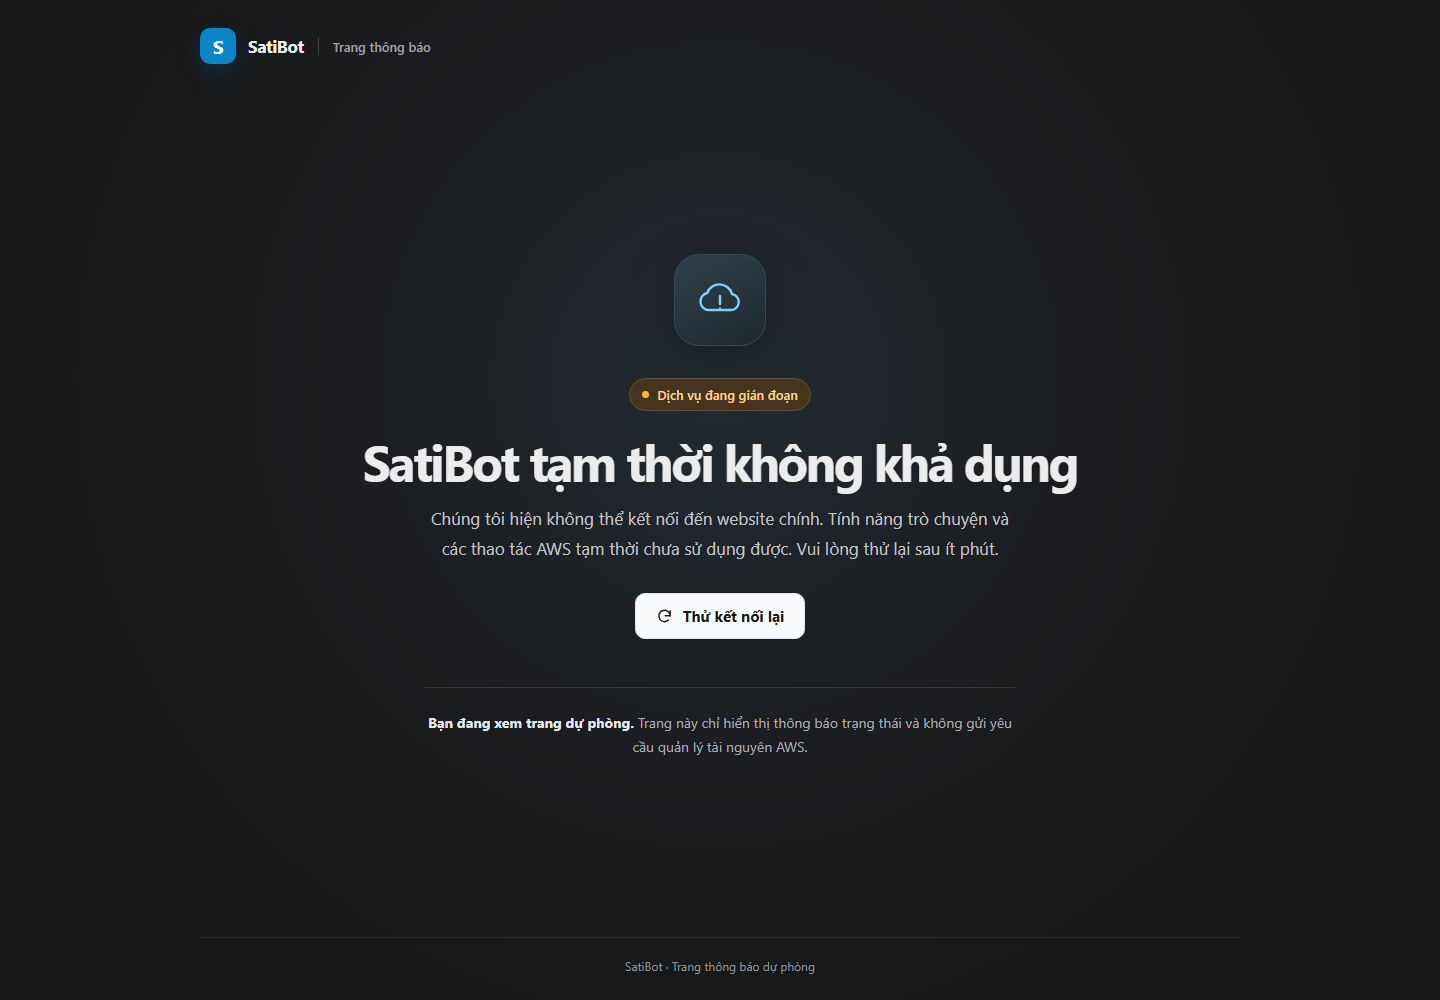
\includegraphics[width=0.9\linewidth,height=0.30\textheight,keepaspectratio]{evidence/sprint4-error-page.png}
\caption{Trang fallback tĩnh phục vụ tự động từ S3 tại \code{us-east-1} khi origin chính gặp sự cố \code{504}}
\label{fig:sprint4-error-page}
\end{figure}

\subsection{Nghiệm thu các kịch bản quản trị AWS và đánh giá hiệu năng}

\subsubsection{Nghiệm thu sáu kịch bản Amazon S3}

\begingroup
\small
\begin{longtable}{@{}p{0.8cm}p{4.1cm}>{\raggedright\arraybackslash}p{\dimexpr\linewidth-4.9cm-4\tabcolsep\relax}@{}}
\caption{Kết quả nghiệm thu các kịch bản S3 trên website bản thử}\label{tab:s3-acceptance}\\
\toprule
STT & Kịch bản & Kết quả quan sát \\
\midrule
\endfirsthead
\endhead
\endfoot
\bottomrule
\endlastfoot
1 & Tạo bucket an toàn & \textbf{Đạt.}Tạo bucket private thành công tại Singapore, bật đủ Block Public Access. \\
2 & Quét/khóa public access & \textbf{Đạt.} Quét 5 bucket, không phát hiện bucket rủi ro; bật lại đủ bốn cờ chặn cho bucket thử thành công. \\
3 & Xóa có xác nhận & \textbf{Đạt.} Xem nội dung trước khi xóa; xác nhận bằng đúng tên bucket; xóa bucket cùng 2 mục bên trong. \\
4 & Lifecycle & \textbf{Đạt.} Tạo rule cho prefix \texttt{demo/}, chuyển sang \texttt{STANDARD\_IA} sau 30 ngày. \\
5 & Presigned download & \textbf{Đạt.} Link thời hạn 15 phút tải được đúng tệp mẫu, phản hồi HTTP 200. \\
6 & Dung lượng và chi phí & \textbf{Đạt.} Thống kê 2 object, 1.000.038 byte (xấp xỉ 0,001 GB), lớp \texttt{STANDARD}; ước tính 0,000025 USD/tháng. \\
\end{longtable}
\endgroup

Chi phí trong bảng là \textbf{ước tính}
theo đơn giá tham chiếu, không phải hóa đơn AWS; thao tác lifecycle chỉ xác
minh cấu hình rule, chưa chờ đủ 30 ngày để quan sát dịch chuyển storage class.

\subsubsection{Nghiệm thu các kịch bản Amazon EC2}

\subsubsection{Nghiệm thu các kịch bản AWS IAM}

\subsubsection{Nghiệm thu kịch bản quản trị AWS Lambda qua giao diện ChatOps}

Thông qua giao diện chat tiếng Việt trên \url{https://satibot.id.vn/} kết nối bằng vai trò liên kết STS \code{AssumeRole} sang tài khoản AWS đích, nhóm đã kiểm thử toàn bộ \textbf{12/12 công cụ quản trị Lambda} cùng các cơ chế Guardrail an toàn. Toàn bộ kết quả hiển thị trên khung chat khớp hoàn toàn với trạng thái tài nguyên trên AWS Console và được ghi nhận đầy đủ trong bảng \code{ActionHistory} (Bảng~\ref{tab:lambda_acceptance_summary}).

\begingroup
\setlength{\tabcolsep}{6pt}
\renewcommand{\arraystretch}{1.15}
\fontsize{10.5}{14}\selectfont
\begin{longtable}{@{}>{\raggedright\arraybackslash}p{5.1cm}>{\raggedright\arraybackslash}p{\dimexpr\linewidth-5.1cm-2\tabcolsep\relax}@{}}
\caption{Tổng hợp kết quả nghiệm thu các kịch bản và Guardrail quản trị Lambda}\label{tab:lambda_acceptance_summary}\\
\toprule
\textbf{Kịch bản \& Guardrail an toàn} & \textbf{Kết quả thực hiện và đối chiếu thực tế}\\
\midrule
\endfirsthead
\endhead
\endfoot
\bottomrule
\endlastfoot
1. Audit danh sách, config và source code Lambda & \textbf{Đạt.} Liệt kê chính xác toàn bộ các hàm Lambda trong region; đọc đúng \code{runtime}, \code{RAM}, \code{timeout} và tải lại chính xác file mã nguồn Python đang chạy trên AWS.\\
2. Chẩn đoán sức khỏe Lambda (\textit{Health Audit}) & \textbf{Đạt (100/100 điểm).} Tự động phát hiện các hàm cấu hình tài nguyên thấp; sau khi chuẩn hóa RAM $\ge 256$~MB và timeout $\ge 15$~s, cả 7 hàm đều đạt trạng thái \code{HEALTHY} theo bộ tiêu chí kiểm tra cấu hình của công cụ.\\
3. Tạo hàm mới \& \textit{Conflict Guardrail} & \textbf{Đạt.} Tạo thành công hàm Python~3.12 mới với mã nguồn do người dùng/LLM cung cấp. Khi gặp tên hàm đã tồn tại, hệ thống dừng lại yêu cầu chọn hướng xử lý (update, đổi tên, cancel) thay vì tự ý ghi đè.\\
4. \textit{AST Validation Guardrail} trước khi deploy & \textbf{Đạt.} Tự động chặn sớm các lỗi cú pháp, các lời gọi bị cấm theo quy tắc của dự án (\code{eval}/\code{exec}) và việc dùng nhầm các định danh theo cú pháp JSON (\code{true}/\code{false}/\code{null} thay cho \code{True}/\code{False}/\code{None}).\\
5. Update code \& Invoke hàm trực tiếp qua Chat & \textbf{Đạt.} Đóng gói, cập nhật phiên bản code mới và invoke trực tiếp hàm với test payload JSON, trả về HTTP~200 cùng output và execution duration.\\
6. Hot Config tài nguyên (RAM / Timeout) & \textbf{Đạt.} Cập nhật cấu hình bộ nhớ và timeout ngay trên khung chat sau bước xác nhận; cấu hình cập nhật thành công và khớp hoàn toàn trên AWS Console.\\
7. Tạo Function URL \& \textit{CORS Wildcard Guardrail} & \textbf{Đạt.} Từ chối CORS origin \code{*} theo quy tắc của dự án; chỉ cấp phát HTTPS Endpoint công khai khi truyền origin hợp lệ (\url{https://satibot.id.vn}), gọi thử trả HTTP~200. CORS giới hạn truy cập khác origin từ trình duyệt, không thay thế cơ chế xác thực.\\
8. Cấu hình \textit{Resilient Service} (Alias, Async Retry) & \textbf{Đạt.} Tự động publish Version, gán Alias \code{live}, bật Async Retry, đồng thời thực hiện Graceful Degradation kèm warning khi tài khoản chạm giới hạn concurrency.\\
9. \textit{Emergency Kill-Switch} (Throttle) & \textbf{Đạt.} Đặt \code{Reserved Concurrency = 0} ngăn phát sinh lượt thực thi mới; sau đó gỡ bỏ giới hạn để khôi phục hoạt động bình thường.\\
10. \textit{Core Deny Guardrail} \& Delete hàm thử nghiệm & \textbf{Đạt.} Lệnh yêu cầu xóa hàm core của chính SatiBot bị từ chối ở tầng IAM (\code{AccessDenied}); các hàm thử nghiệm được xóa và xác minh không còn tồn tại.\\
\end{longtable}
\endgroup

\subsubsection{Đánh giá hiệu năng vận hành thực tế và bài học tối ưu kỹ thuật}

Qua theo dõi CloudWatch Logs trên tổng số \textbf{1.125 lượt invoke} (gồm \textbf{144 Cold Start} và \textbf{981 Warm Start}), cùng 144 lần chạy Step Functions workflow, hệ thống vận hành ổn định và không ghi nhận bất kỳ Unhandled Exception / Traceback nào (Bảng~\ref{tab:lambda_performance}).

\begingroup
\setlength{\tabcolsep}{5pt}
\renewcommand{\arraystretch}{1.15}
\fontsize{10}{13.5}\selectfont
\begin{longtable}{@{}>{\raggedright\arraybackslash}p{2.6cm}>{\centering\arraybackslash}p{2.4cm}>{\raggedright\arraybackslash}p{3.0cm}>{\raggedright\arraybackslash}p{\dimexpr\linewidth-8.0cm-6\tabcolsep\relax}@{}}
\caption{Hiệu năng vận hành thực tế của 6 hàm AWS Lambda trong hệ thống SatiBot}\label{tab:lambda_performance}\\
\toprule
\textbf{Hàm Lambda} & \textbf{RAM / Timeout} & \textbf{Invoke \& Cold Start} & \textbf{Init Duration, Latency \& Đặc điểm vận hành}\\
\midrule
\endfirsthead
\endhead
\endfoot
\bottomrule
\endlastfoot
\code{Chatbot} & 256~MB / 60~s & 273 lượt (25 cold) & Init 128--181~ms; latency TB $\sim 3{,}1$~s (chủ yếu do chờ API Gemini LLM); Peak RAM 107~MB.\\
\code{Dispatcher} & 512~MB / 60~s & 138 lượt (19 cold) & Init 272--394~ms; latency TB $\sim 2{,}1$~s (gồm lấy credential tạm qua STS và gọi Boto3 đa tài khoản); Peak RAM 255~MB.\\
\code{Formatter} & 256~MB / 30~s & 132 lượt (17 cold) & Init 81--112~ms; latency TB $\sim 3{,}1$~s (chờ Gemini tổng hợp và phát AppSync GraphQL); Peak RAM 96~MB.\\
\code{Connector} & 256~MB / 30~s & 94 lượt (32 cold) & Init 297--398~ms; latency TB $\sim 0{,}5$~s (kiểm tra kết nối STS và ghi cấu hình DynamoDB); Peak RAM 93~MB.\\
\code{History} & 256~MB / 30~s & 403 lượt (18 cold) & Init 254--372~ms; Warm \textbf{2--9~ms} (TB 76~ms) khi query DynamoDB; Peak RAM 92~MB.\\
\code{HealthCheck} & 256~MB / 15~s & 85 lượt (33 cold) & Init 66--101~ms; Warm \textbf{1--2~ms} (TB 7,6~ms) phục vụ Route~53 Health Check; Peak RAM 33~MB.\\
\end{longtable}
\endgroup

Từ số liệu đo đạc thực tế, nhóm rút ra ba điểm cải tiến kỹ thuật cốt lõi đã được kiểm chứng và đưa vào hệ thống vận hành:
\begin{enumerate}[itemsep=3pt,topsep=2pt]
  \item \textbf{Phân tách rõ Latency Bottleneck:} Tầng serverless nội bộ phản hồi rất nhanh ở trạng thái Warm (\textbf{2--9~ms} ở \code{History} và \textbf{1--2~ms} ở \code{HealthCheck}); Chatbot và Formatter có latency trung bình khoảng 3,1 giây mỗi hàm, chủ yếu do gọi Gemini LLM API, nên kiến trúc bất đồng bộ Step Functions kết hợp AppSync WebSocket giúp UI không bị block trong lúc chờ xử lý.
  \item \textbf{Giới hạn mức tăng bộ nhớ của \code{Dispatcher} cache:} Phân tích CloudWatch Logs phát hiện bộ nhớ sử dụng tăng dần khi lưu các session/client phục vụ STS \code{AssumeRole} tới sát ngưỡng 255/256~MB sau khoảng 10 lần gọi liên tiếp. Nhóm đã giới hạn kích thước cache tối đa 8 session, tái sử dụng \code{boto3.client} dùng chung tài nguyên và chuẩn hóa nâng RAM của \code{Dispatcher} lên \textbf{512~MB} qua CI/CD pipeline.
  \item \textbf{\textit{AST Guardrail} khắc phục lỗi sinh code của LLM:} Bổ sung các quy tắc kiểm tra trên AST trước khi đóng gói giúp phát hiện việc dùng nhầm các định danh theo cú pháp JSON (\code{true}/\code{false}/\code{null}) và gợi ý sửa về chuẩn Python (\code{True}/\code{False}/\code{None}), nâng độ ổn định khi tạo và cập nhật Lambda bằng ngôn ngữ tự nhiên.
\end{enumerate}

\subsection{Vai trò và đóng góp của các thành viên}

\begingroup
\setlength{\tabcolsep}{6pt}
\renewcommand{\arraystretch}{1.15}
\fontsize{10.5}{14}\selectfont
\begin{longtable}{@{}>{\raggedright\arraybackslash}p{4.0cm}>{\raggedright\arraybackslash}p{\dimexpr\linewidth-4.0cm-2\tabcolsep\relax}@{}}
\caption{Phân công và kết quả đóng góp của Nhóm 10}\label{tab:team-roles}\\
\toprule
\textbf{Thành viên} & \textbf{Vai trò phụ trách và kết quả bàn giao} \\
\midrule
\endfirsthead
\endhead
\endfoot
\bottomrule
\endlastfoot
Cao Anh Minh \textbf{(Trưởng nhóm)} & Thiết kế kiến trúc tổng thể, phân quyền IAM, mô hình 5 bảng DynamoDB, điều phối tích hợp đa dịch vụ (Step Functions, AppSync, nền tảng CDK Data/IAM) và tổng hợp báo cáo. \\
Trịnh Thiên Quang & Phát triển cụm 5 Lambda backend, tích hợp Gemini API, thiết lập CI/CD Pipeline (\textit{CodePipeline/CodeDeploy Canary}), tối ưu memory cache và nghiệm thu 12/12 công cụ quản trị AWS Lambda. \\
Phạm Đức Hùng & Xây dựng module quản trị và nghiệm thu 6 kịch bản Amazon S3; phát triển giao diện React, kết nối frontend AppSync, cấu hình AWS WAF và trang fallback tại \code{us-east-1}. \\
Nguyễn Đức Huy & Xây dựng module quản trị Amazon EC2, lớp xác thực Amazon Cognito / API Gateway, cấu hình tên miền \code{satibot.id.vn}, chứng chỉ ACM và định tuyến Route~53 Health Check / Failover. \\
\end{longtable}
\endgroup

\subsection{Liên kết sản phẩm, tài liệu bổ trợ và kết luận}

\begin{itemize}[itemsep=3pt,topsep=2pt]
  \item \textbf{Ứng dụng đã triển khai:} \url{https://satibot.id.vn/} (API Health Check: \url{https://api.satibot.id.vn/api/health}).
  \item \textbf{Mã nguồn GitHub:} \url{https://github.com/minhcaoj/SitaBot}.
  \item \textbf{Slide báo cáo cuối kỳ:} \textit{[Bổ sung đường dẫn slide khi nộp bài]}.
  \item \textbf{Video trình bày và demo hệ thống:} \textit{[Bổ sung đường dẫn video sau khi quay và tải lên]}.
  \item \textbf{Tài liệu bổ trợ \& Nhật ký công việc:} Báo cáo Progress~1, Progress~2, bộ test tự động (\path{tests/}, \path{frontend/}), dữ liệu đối chiếu WAF (\path{evidence/}) và lịch sử commit/Pull Request trên GitHub (biên bản họp nhóm đính kèm khi nộp).
\end{itemize}

\noindent\textbf{Kết luận.} Nhóm đã triển khai và đưa vào vận hành hoàn chỉnh hệ thống SatiBot tại \url{https://satibot.id.vn/} với hạ tầng khai báo bằng AWS CDK, backend tại region chính và trang thông báo dự phòng tại region thứ hai, quy trình CI/CD kết hợp CodeDeploy Canary từ GitHub lên AWS có bước phê duyệt thủ công, lớp bảo mật biên WAF và Origin Failover hoạt động ổn định, cùng phân hệ quản trị ChatOps an toàn qua AWS Lambda và Amazon S3.

\end{document}
